\documentclass[10pt,a4paper,titlepage]{article}
\usepackage[utf8]{inputenc}
\usepackage{amsmath}
\usepackage{amsfonts}
\usepackage{amssymb}
\usepackage{graphicx}
\usepackage{subcaption}
\usepackage{float}
\usepackage{tabularx}
%\usepackage{mwe}
\author{Claude Goubet}
\title{Project technical report 1}
\begin{document}
\maketitle


\section{Previous works}
	See literature file.

\section{Data Characteristics}

Parameters defining the projection file format

\begin{itemize}
	\item number of projections: 2000
	\item image dimensions: $2048 \times 20148$
	\item vertical and horizontal pixel size: 0.119865 microns
\end{itemize}

Parameters defining experiment

\begin{itemize}


	\item angle between projections: 0.09 degree
	\item Vertical rotation axis position: 1024.006591 pixel
	\item energy: 33.6
\end{itemize}

Parameters defining reconstruction

\begin{itemize}
	\item start voxel: (1,1,1) end voxel (2048, 2048, 256) of reconstruction volume
	\item Optic used: 0.119865	
	\item Pad method: reflect
	\item number of planes: 4
	\item number of angles: 645
	\item Rotation axis
	\item ...
	
\end{itemize}
\clearpage
\section{Reading The Data}
	\subsection{Projections}
		show 4 different projection out of 100
	\subsection{Sinogram}
		From the projections by taking one row in each projection we were able to reconstruct a sinogram as in Frigure \ref{fig:Sino}\\
		Individual images are displayed in the index section \ref{SinoImg}
		\begin{figure}[H]
    		\centering
		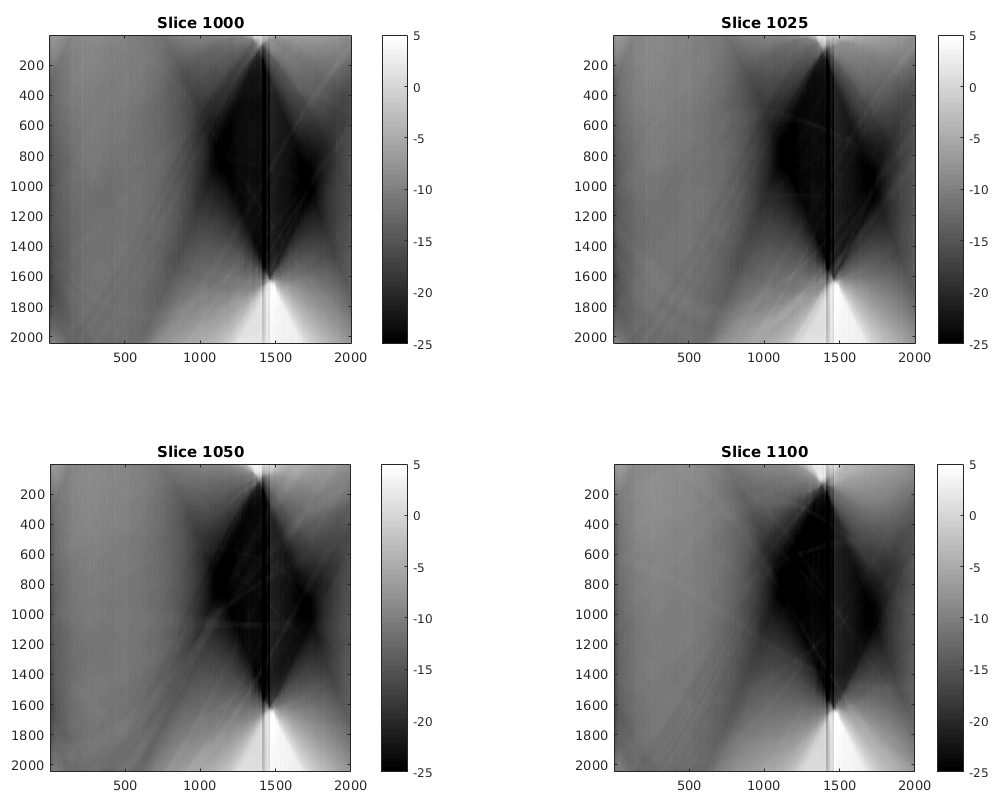
\includegraphics[width=1.1\textwidth]{sinograms/Sinograms2.png}	
			\caption{Sinogram of slice 1000, 1025, 1050, 1100}
    	\label{fig:Sino}
		
		\end{figure}

	\clearpage
\section{FBP Reconstruction}
	In this section we try multiple FBP parameters in order to understand their influence on the reconstruction. We took as input the sinograms diplayed previously.
	\subsection{Reconstruction without zero-padding default filter}
		We first performed the MatLab default iradon function for the reconstruction without trying to correct the center of rotation of the object.\\
		The resulting images (Figure \ref{fig:wtout0pad}) are subjected to artefacts particularly on corner details.\\
		 Full images refer to Index \ref{wtout0pad}
		 
		\begin{figure}[H]
		
        \centering
        \begin{subfigure}[b]{0.475\textwidth}
            \centering
            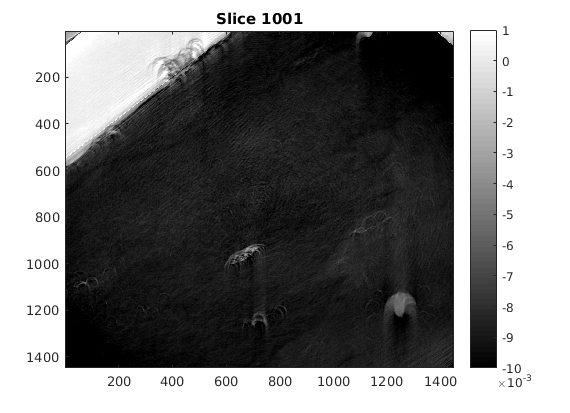
\includegraphics[width=\textwidth]{no0pad/slice1001.png}
            %\caption[Network2]%
            %{{\small Network 1}}    
            \label{fig:mean and std of net14}
        \end{subfigure}
        \hfill
        \begin{subfigure}[b]{0.475\textwidth}  
            \centering 
            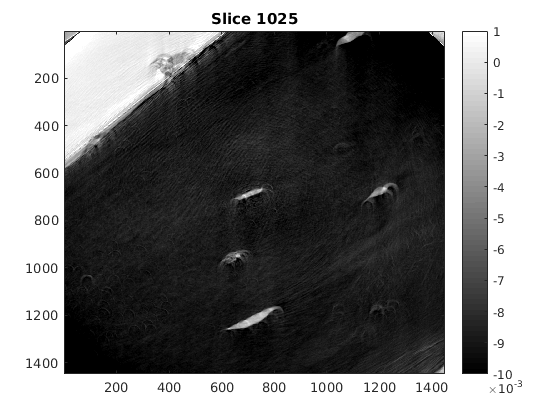
\includegraphics[width=\textwidth]{no0pad/slice1025.png}
            %\caption[]%
            %{{\small Network 2}}    
            \label{fig:mean and std of net24}
        \end{subfigure}
        \vskip\baselineskip
        \begin{subfigure}[b]{0.475\textwidth}   
            \centering 
            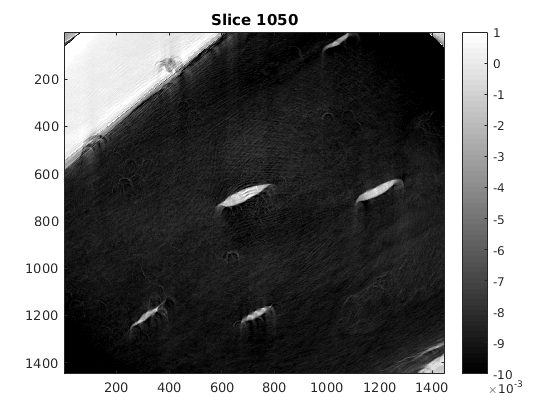
\includegraphics[width=\textwidth]{no0pad/slice1050.png}
            %\caption[]%
            %{{\small Network 3}}    
            \label{fig:mean and std of net34}
        \end{subfigure}
        \quad
        \begin{subfigure}[b]{0.475\textwidth}   
            \centering 
            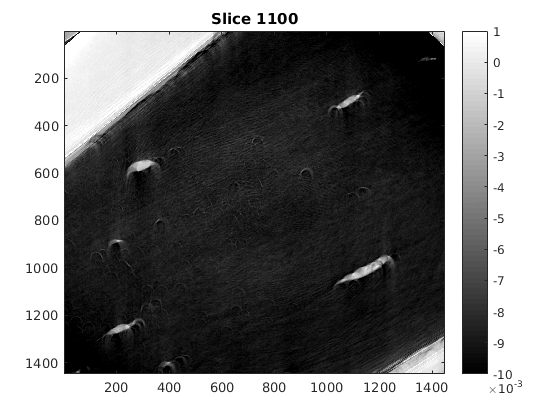
\includegraphics[width=\textwidth]{no0pad/slice1100.png}
            %\caption[]%
            %{{\small Network 4}}    
            \label{fig:mean and std of net44}
        \end{subfigure}
        \caption{FBP without zero-padding}
        \label{fig:wtout0pad}
    \end{figure}
   
    
    \clearpage
	\subsection{Reconstruction with zero-padding}
	
		\subsection{Zero-padding on 4 slices}
			In order to get better images we had to correct the center of rotation. To do so we used the actual rotation axis od $1043.5$ end defined a new output size of $round(2*rotAxis)$. The resulting new sized projections were used to build the new images. The results were non blurry images as is Figure \ref{ZeroPadd}.
			
			\begin{figure}[h!]
        \centering	
			\begin{subfigure}[b]{0.475\textwidth}
            \centering
            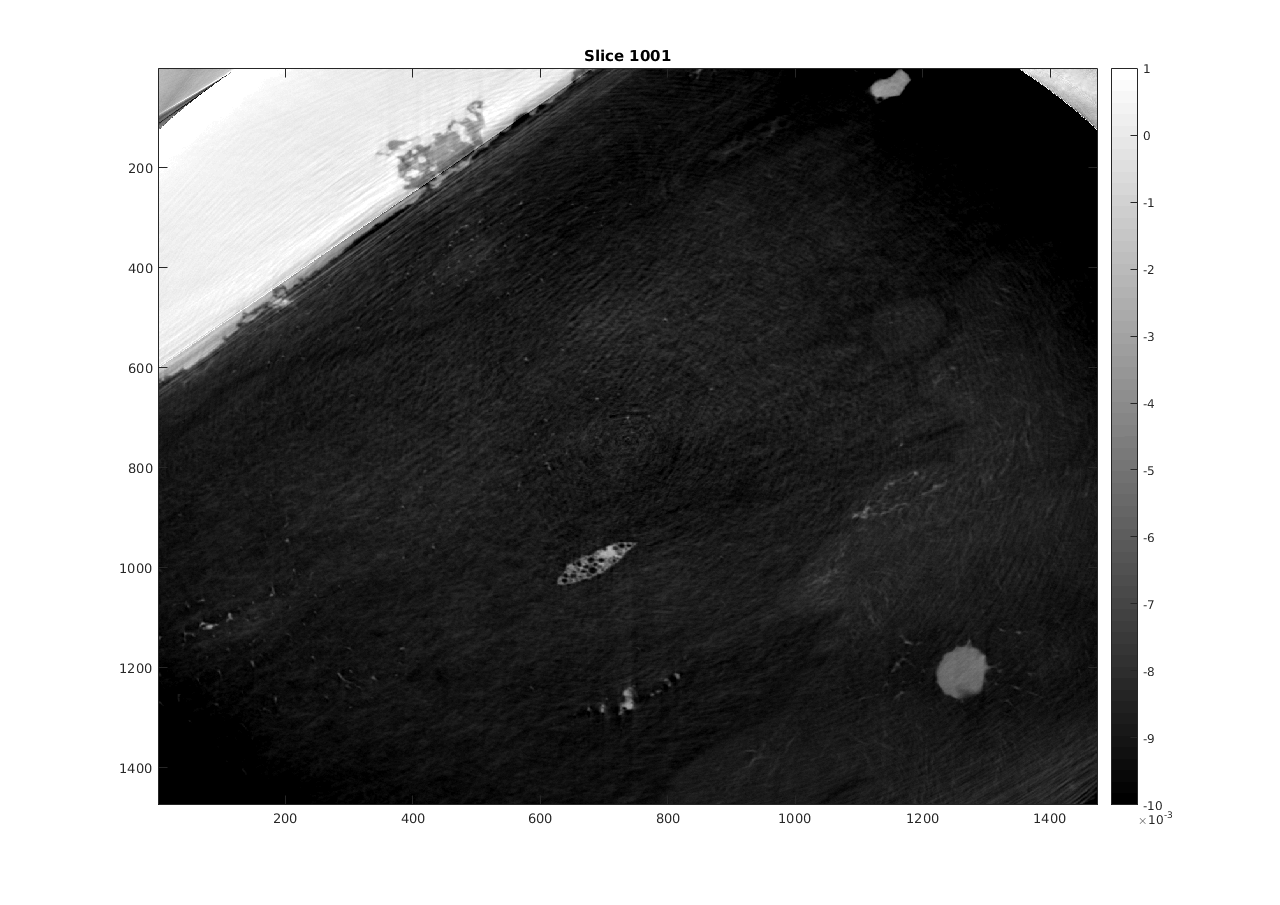
\includegraphics[width=\textwidth]{with0pad/slice1001.png}
            %\caption[Network2]%
            %{{\small Network 1}}    
            \caption{slice 1001}
        \end{subfigure}
        \hfill
        \begin{subfigure}[b]{0.475\textwidth}  
            \centering 
            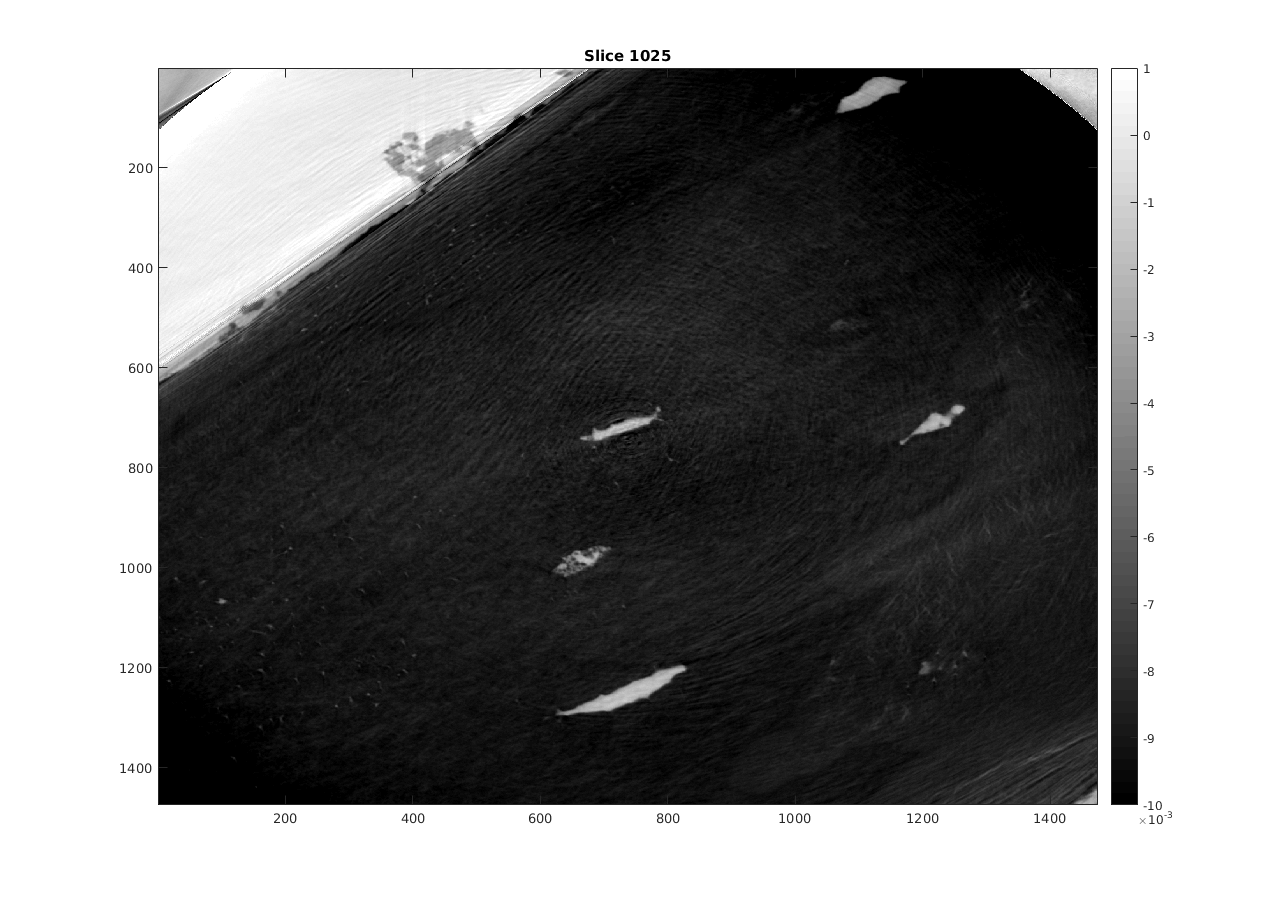
\includegraphics[width=\textwidth]{with0pad/slice1025.png}
            %\caption[]%
            %{{\small Network 2}}    
            \caption{slice 1025}
        \end{subfigure}
        \vskip\baselineskip
        \begin{subfigure}[b]{0.475\textwidth}   
            \centering 
            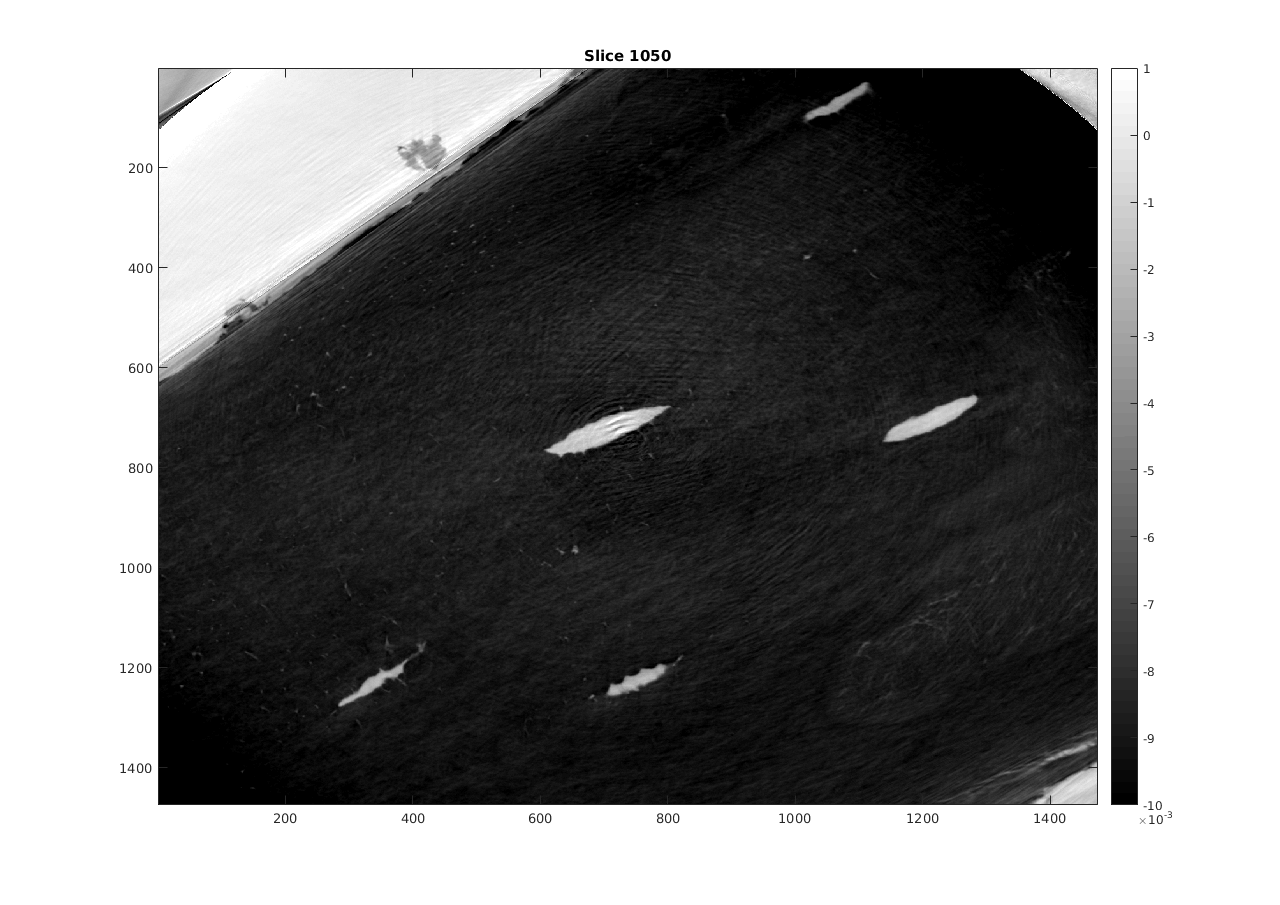
\includegraphics[width=\textwidth]{with0pad/slice1050.png}
            %\caption[]%
            %{{\small Network 3}}    
            \caption{slice 1050}
        \end{subfigure}
        \quad
        \begin{subfigure}[b]{0.475\textwidth}   
            \centering 
            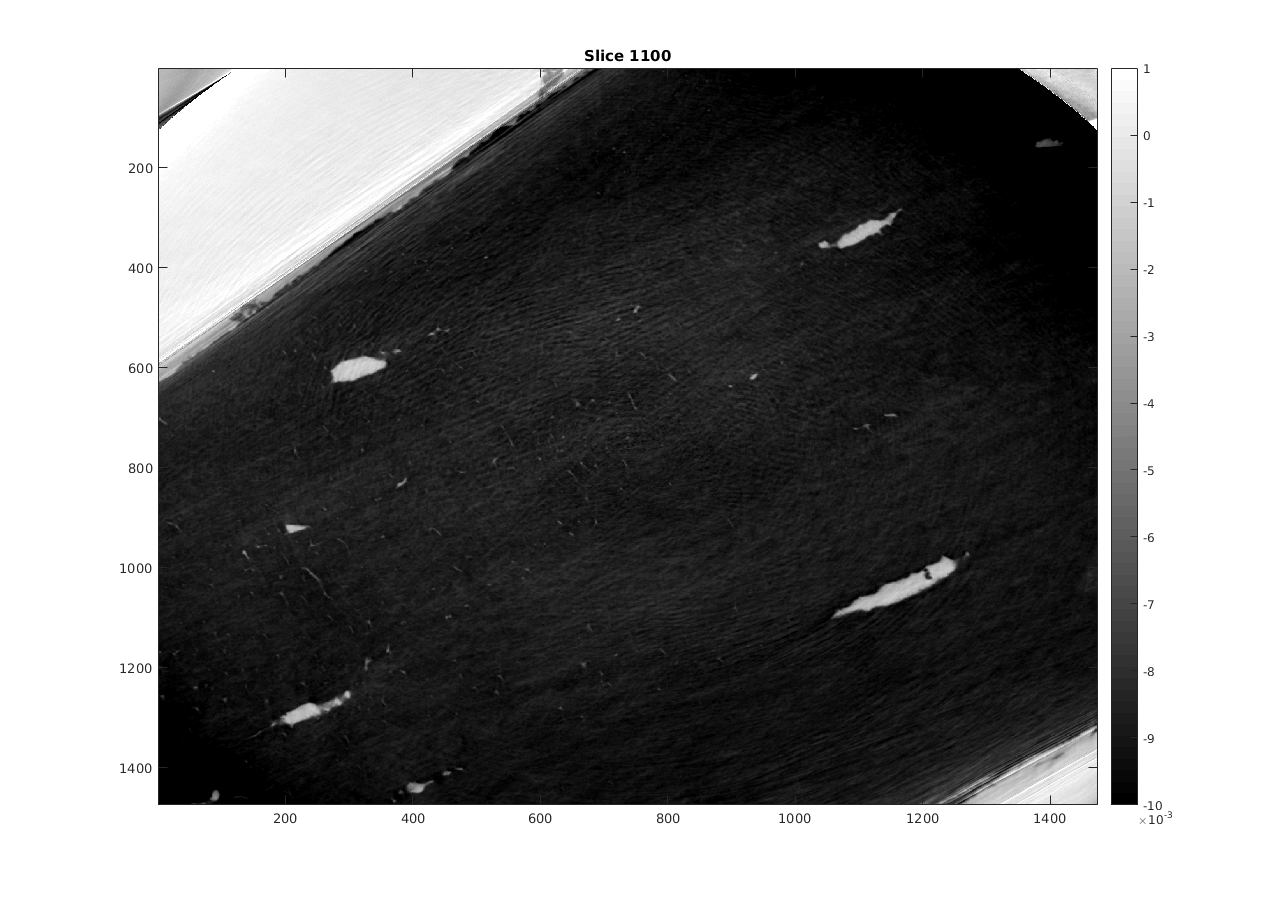
\includegraphics[width=\textwidth]{with0pad/slice1100.png}
            %\caption[]%
            %{{\small Network 4}}    
            \caption{slice 1100}
        \end{subfigure}
        \caption{Back-projection with zero-padding with 2000 projections}
        \label{ZeroPadd}
        \end{figure}
        
	\clearpage
	
	
	
	
	
	\subsubsection{Comparing frequency scaling one slice}
			In this section the fastest filter was used (Ram-Lak) and multiple frequencies were displayed. Low frequencies were affected by a strong ring artifact effect as shown Figure \ref{fig:freq}. Frequencies from 0.7 to 1 were less affected by ring artifact. A frequency of 0.7 was use for the next experiments. 
			
			\begin{figure}[h!]
        \centering	
			\begin{subfigure}[b]{0.475\textwidth}
            \centering
            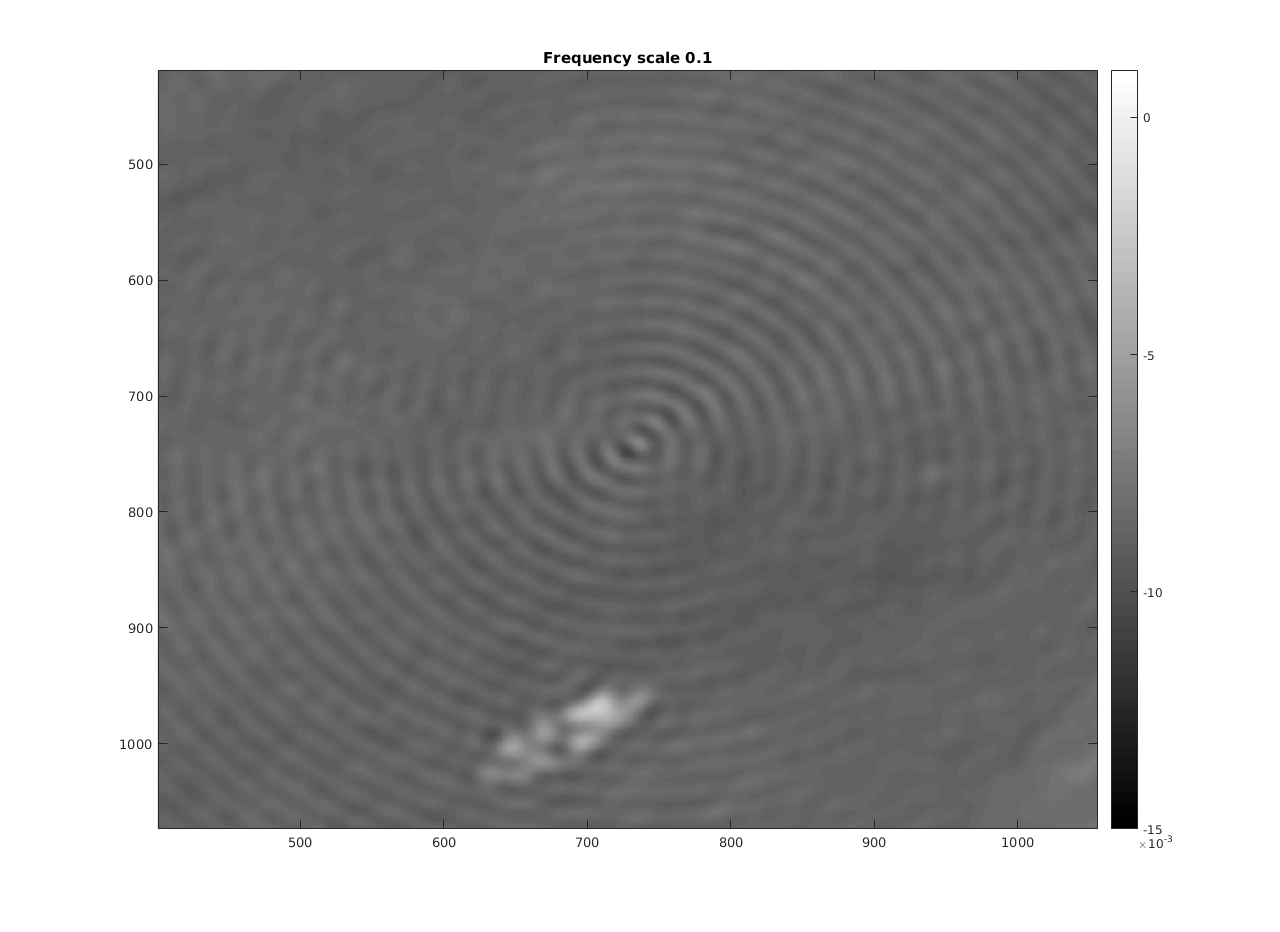
\includegraphics[width=\textwidth]{freq/zoomed/f001.png}  
            \caption{frequency 0.1} 
            \label{freq01}
        \end{subfigure}
        \hfill
        \begin{subfigure}[b]{0.475\textwidth}  
            \centering 
            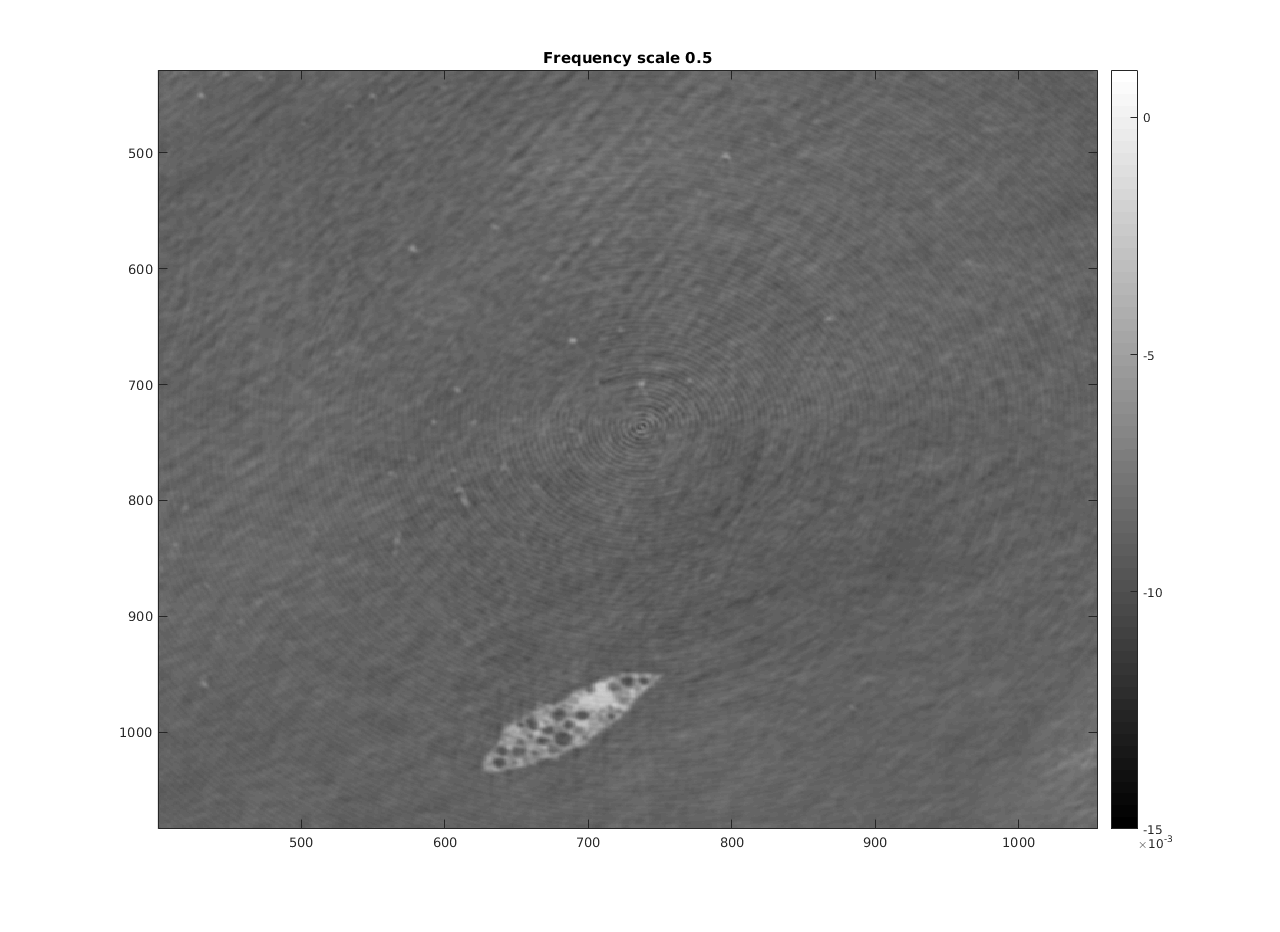
\includegraphics[width=\textwidth]{freq/zoomed/f005.png}   
            \caption{frequency 0.5}
            \label{freq05}
        \end{subfigure}
        \vskip\baselineskip
        \begin{subfigure}[b]{0.475\textwidth}   
            \centering 
            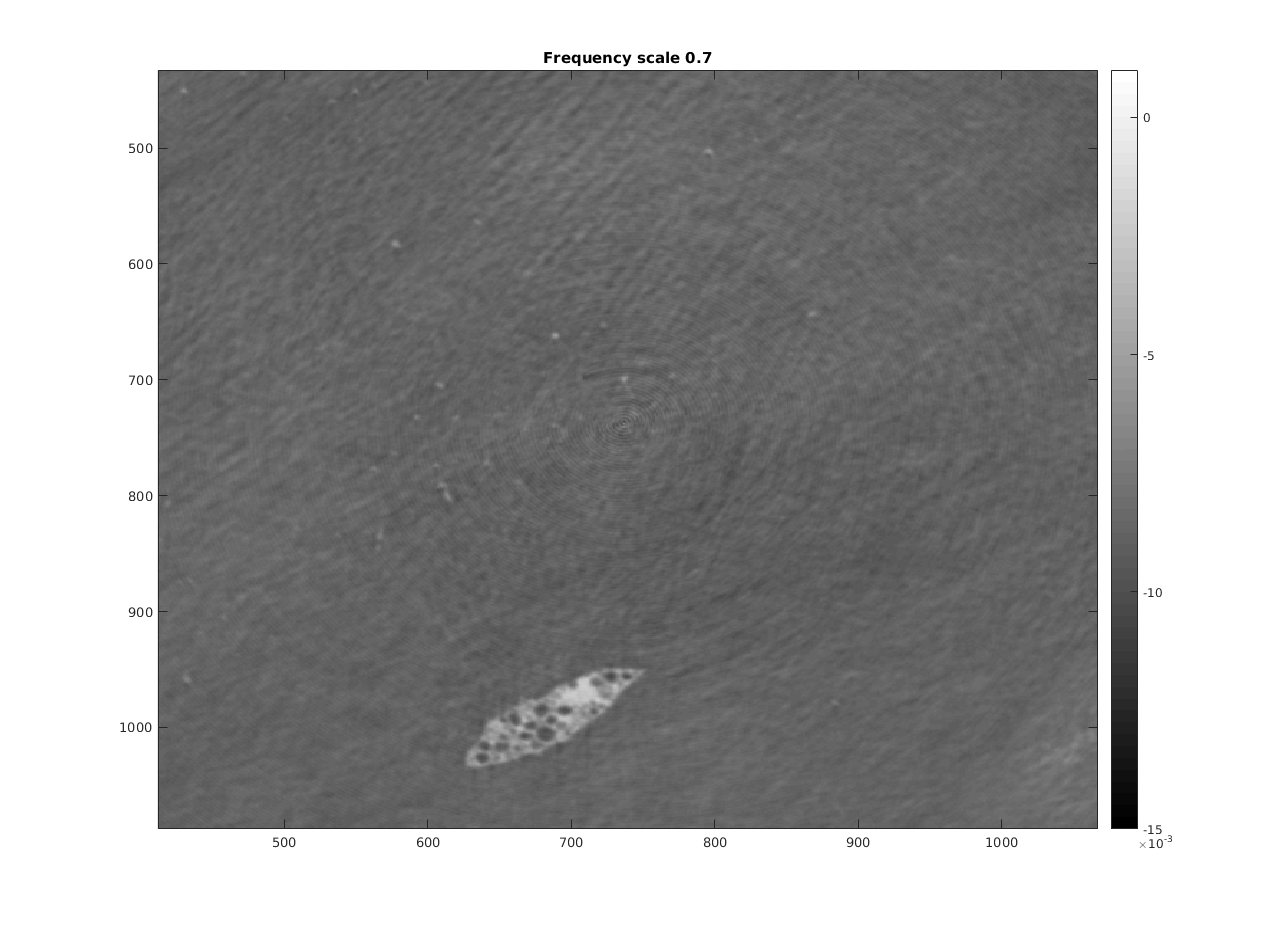
\includegraphics[width=\textwidth]{freq/zoomed/f007.png}  
            \caption{frequency 0.7}
            \label{freq07}
        \end{subfigure}
        \quad
        \begin{subfigure}[b]{0.475\textwidth}   
            \centering 
            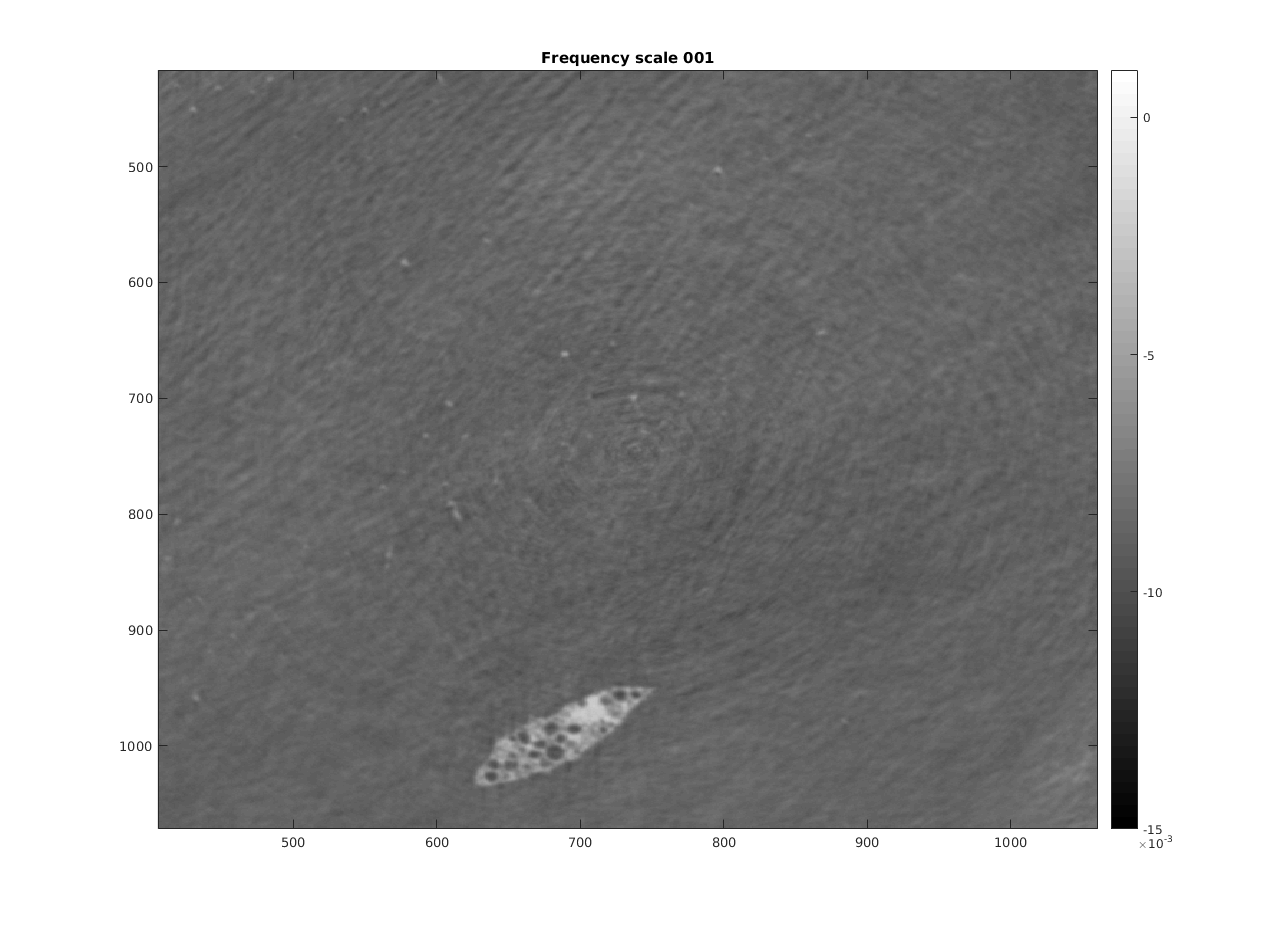
\includegraphics[width=\textwidth]{freq/zoomed/f010.png}   
            \caption{frequency 1}
            \label{freq10}
        \end{subfigure}
        \caption{Multiple frequences for FBP with 2000 projections Slice 1001}
        \label{fig:freq}
    \end{figure}
    
	\clearpage
	
	
		\subsubsection{Using MatLab implemented filters}
			
			Now that we have a correct reconstruction we reconstructed using different filters available on MatLab. As expected FBP without filtering results in a very blurry image with no details Figure \ref{NoFilter}. Figures \ref{Hamming}, \ref{Hann}, \ref{Cosine}, \ref{Ram-Lak} and \ref{Shepp-Logan} Represent a zoomed reconstruction using different filters. We observed similar results. Only computation time was significantly different between each Filter.
			
		\begin{figure}[h!]
        \centering	
			\begin{subfigure}[b]{0.475\textwidth}
            \centering
            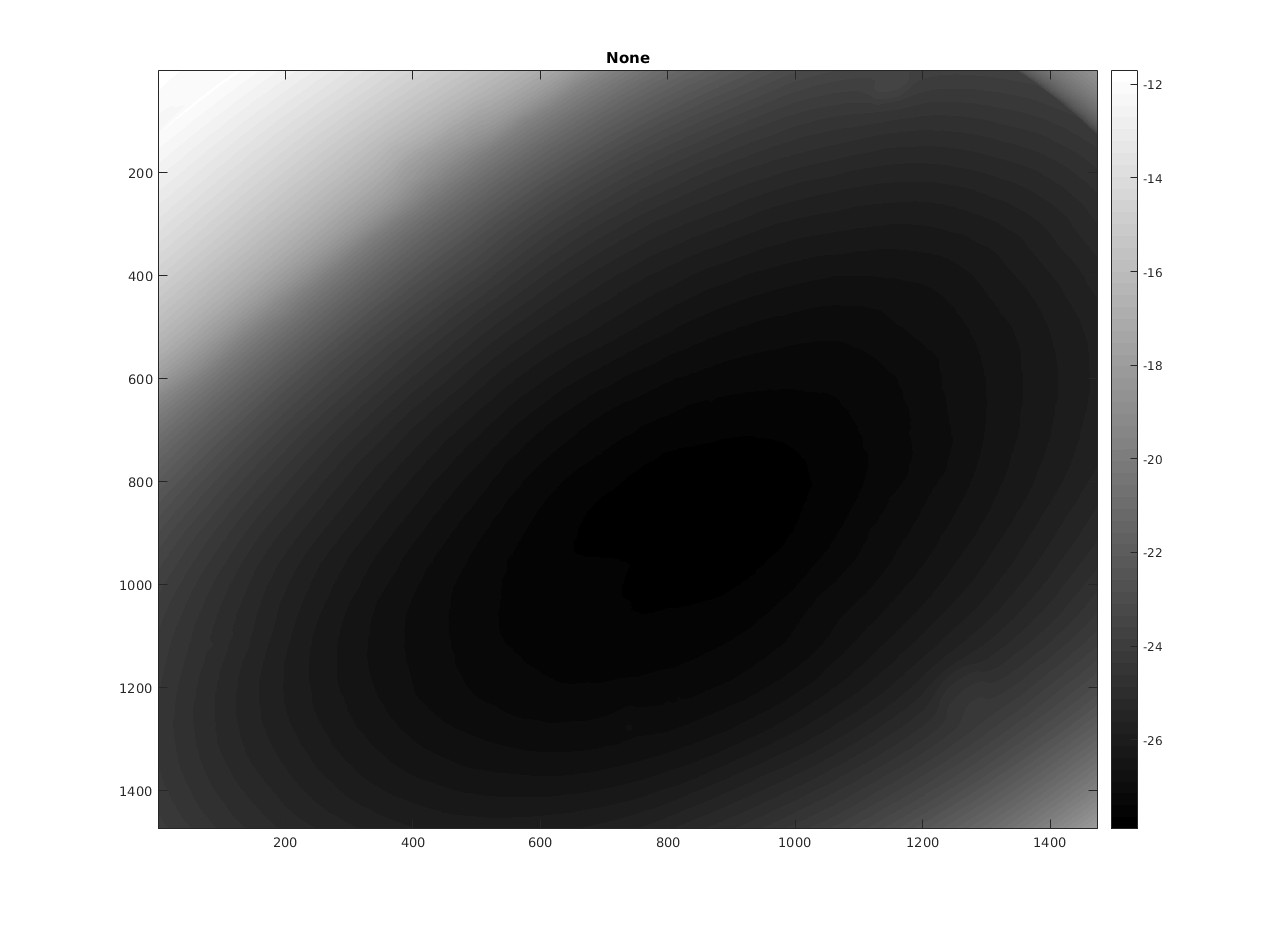
\includegraphics[width=\textwidth]{filters/none.png}  
            \caption{no filtering} 
            \label{NoFilter}
        \end{subfigure}
        \hfill
        \begin{subfigure}[b]{0.475\textwidth}  
            \centering 
            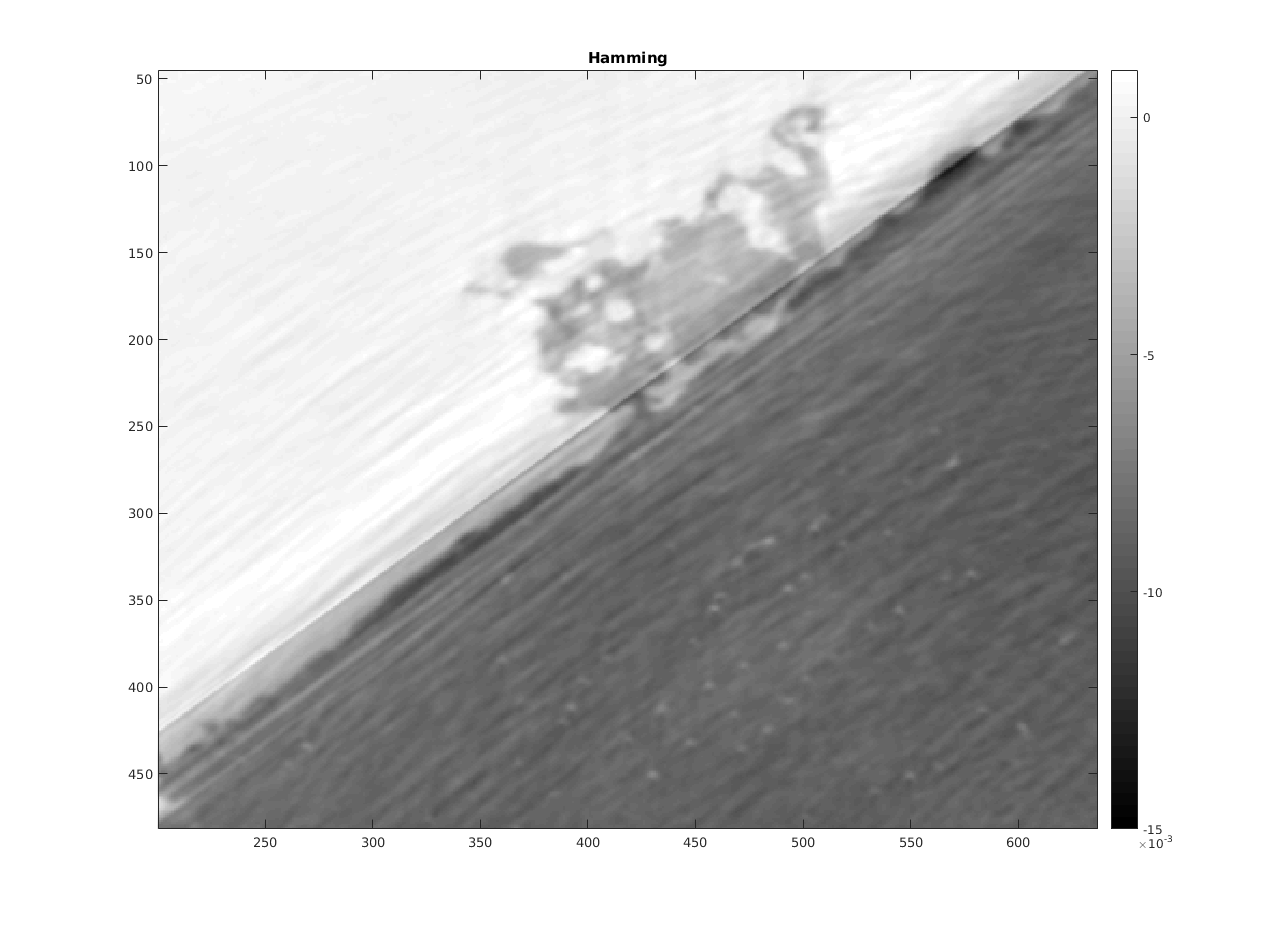
\includegraphics[width=\textwidth]{filters/ZOOMED/Hamming.png}   
            \caption{Hamming}
            \label{Hamming}
        \end{subfigure}
        \vskip\baselineskip
        \begin{subfigure}[b]{0.475\textwidth}   
            \centering 
            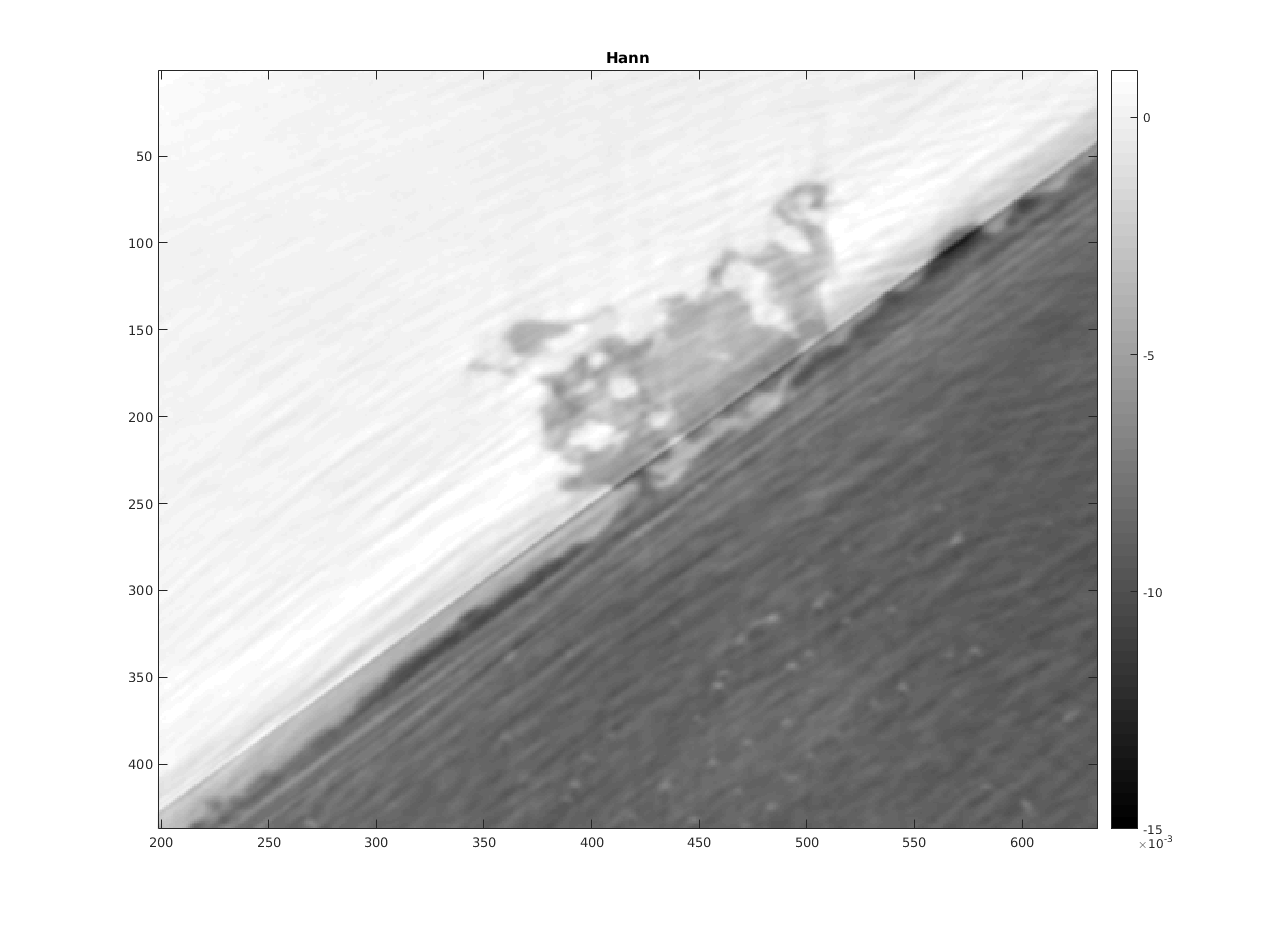
\includegraphics[width=\textwidth]{filters/ZOOMED/Hann.png}  
            \caption{Hann}
            \label{Hann}
        \end{subfigure}
        \quad
        \begin{subfigure}[b]{0.475\textwidth}   
            \centering 
            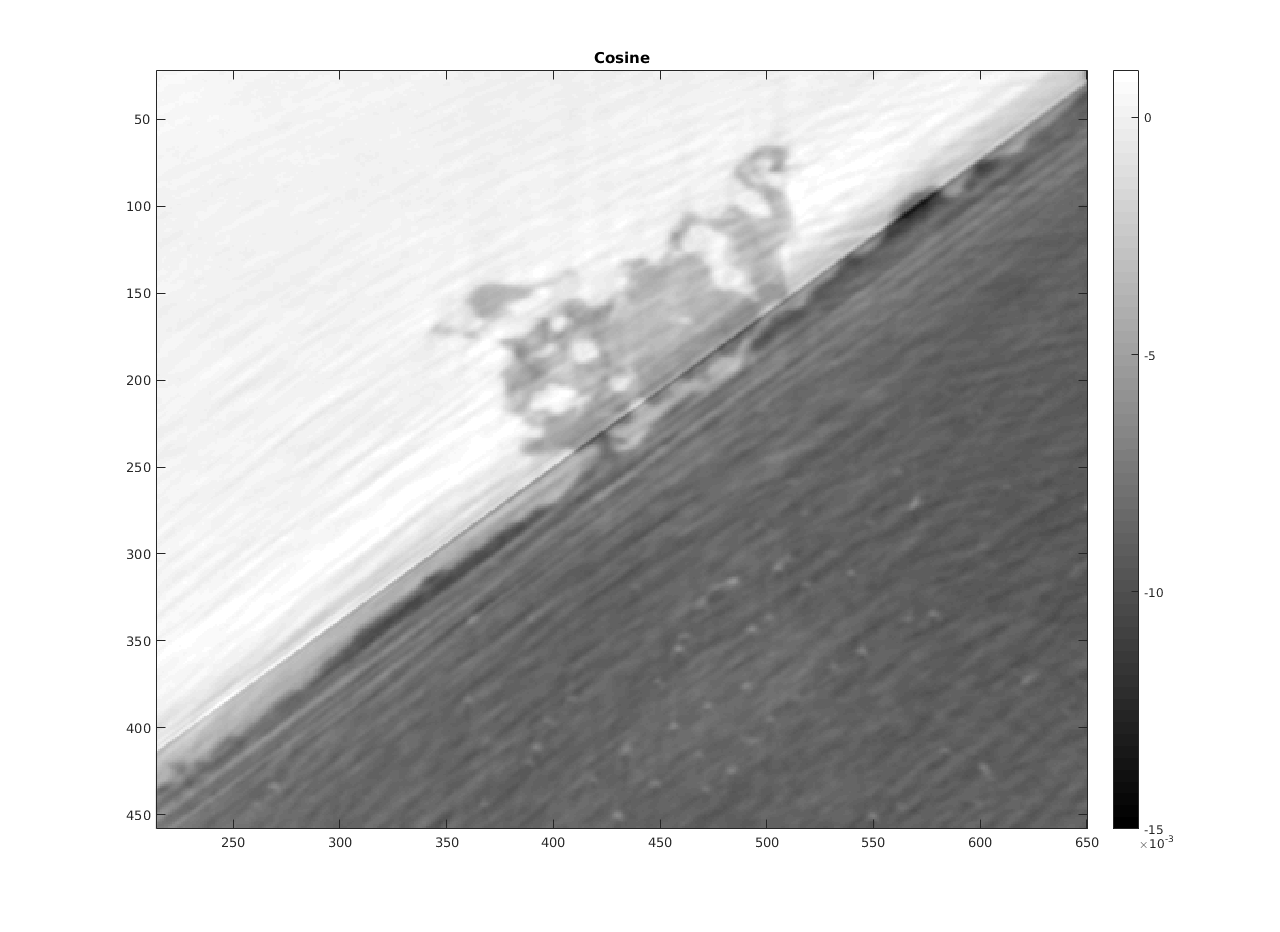
\includegraphics[width=\textwidth]{filters/ZOOMED/Cosine.png}   
            \caption{Cosine}
            \label{Cosine}
        \end{subfigure}
        
         \vskip\baselineskip
        \begin{subfigure}[b]{0.475\textwidth}   
            \centering 
            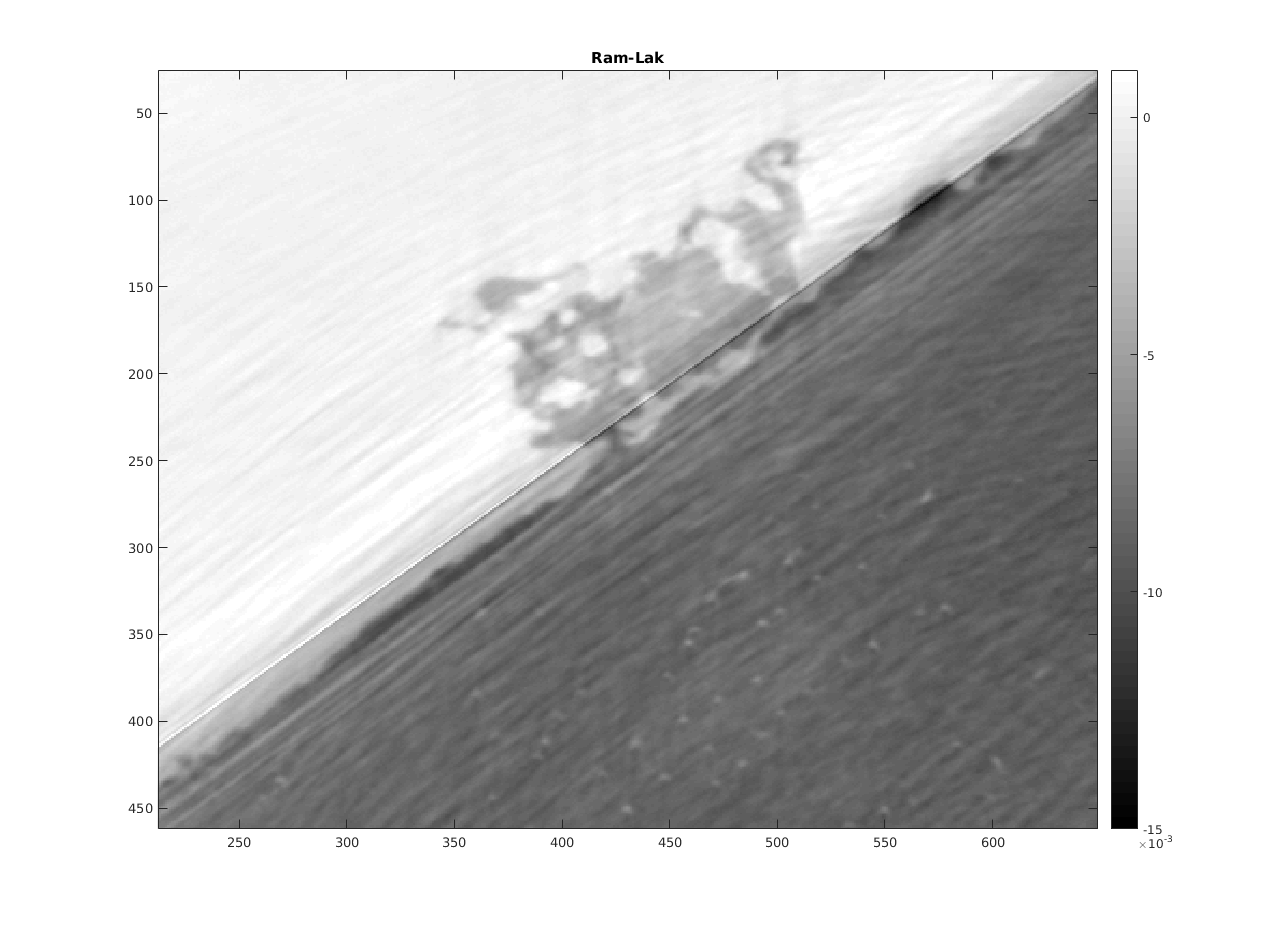
\includegraphics[width=\textwidth]{filters/ZOOMED/Ram-Lak.png}   
            \caption{Ram-Lak}
            \label{Ram-Lak}
        \end{subfigure}
        \quad
        \begin{subfigure}[b]{0.475\textwidth}   
            \centering 
            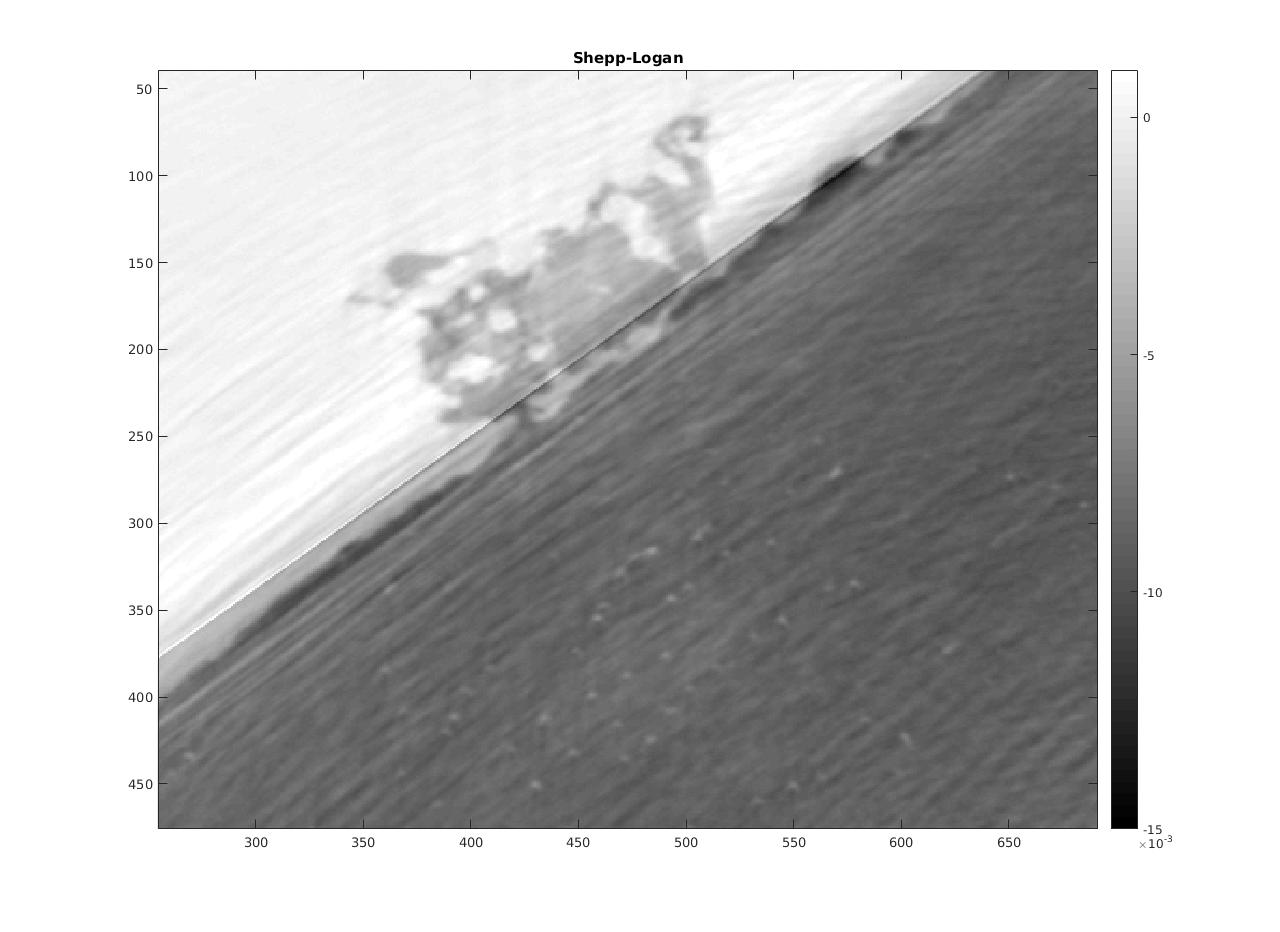
\includegraphics[width=\textwidth]{filters/ZOOMED/Shepp-Logan.png}
            \caption{Shepp-Logan}
            \label{Shepp-Logan}
        \end{subfigure}
        \caption{Multiple filters for FBP with 2000 projections Slice 1001}
        \label{fig:filters}
    \end{figure}
    
    \clearpage




		\subsubsection{Comparing matlab implemented interpolation methods}
			All of the interpolation methods proposed bu irandon MatLab function were used and compared. Once again all reconstructions resulted in the same results. Only the computation time changed.
			
		\begin{figure}[h!]
        \centering	
			\begin{subfigure}[b]{0.475\textwidth}
            \centering
            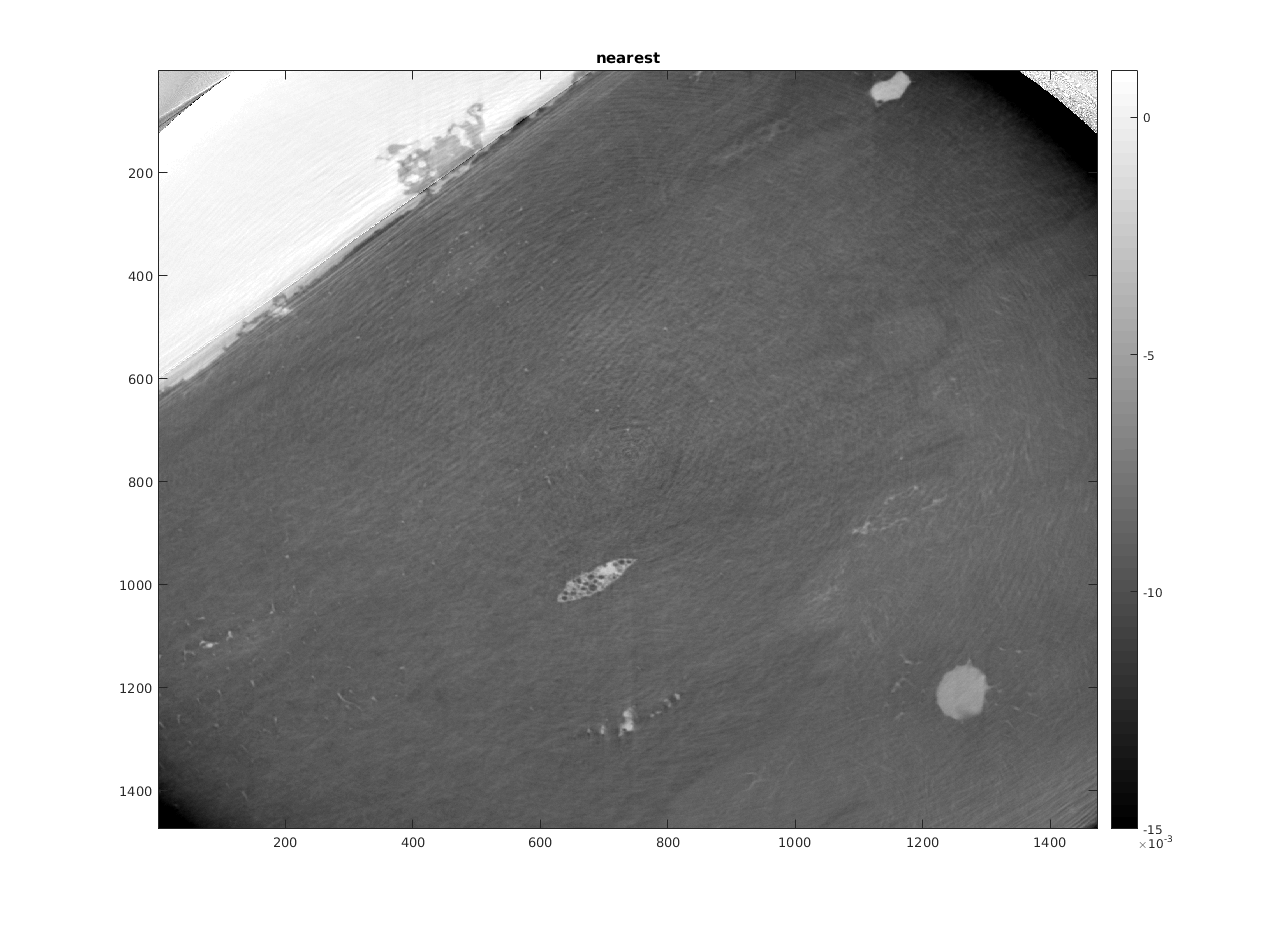
\includegraphics[width=\textwidth]{interp/nearest.png}  
            \caption{Nearest-neighbor interpolation} 
            \label{nearest}
        \end{subfigure}
        \hfill
        \begin{subfigure}[b]{0.475\textwidth}  
            \centering 
            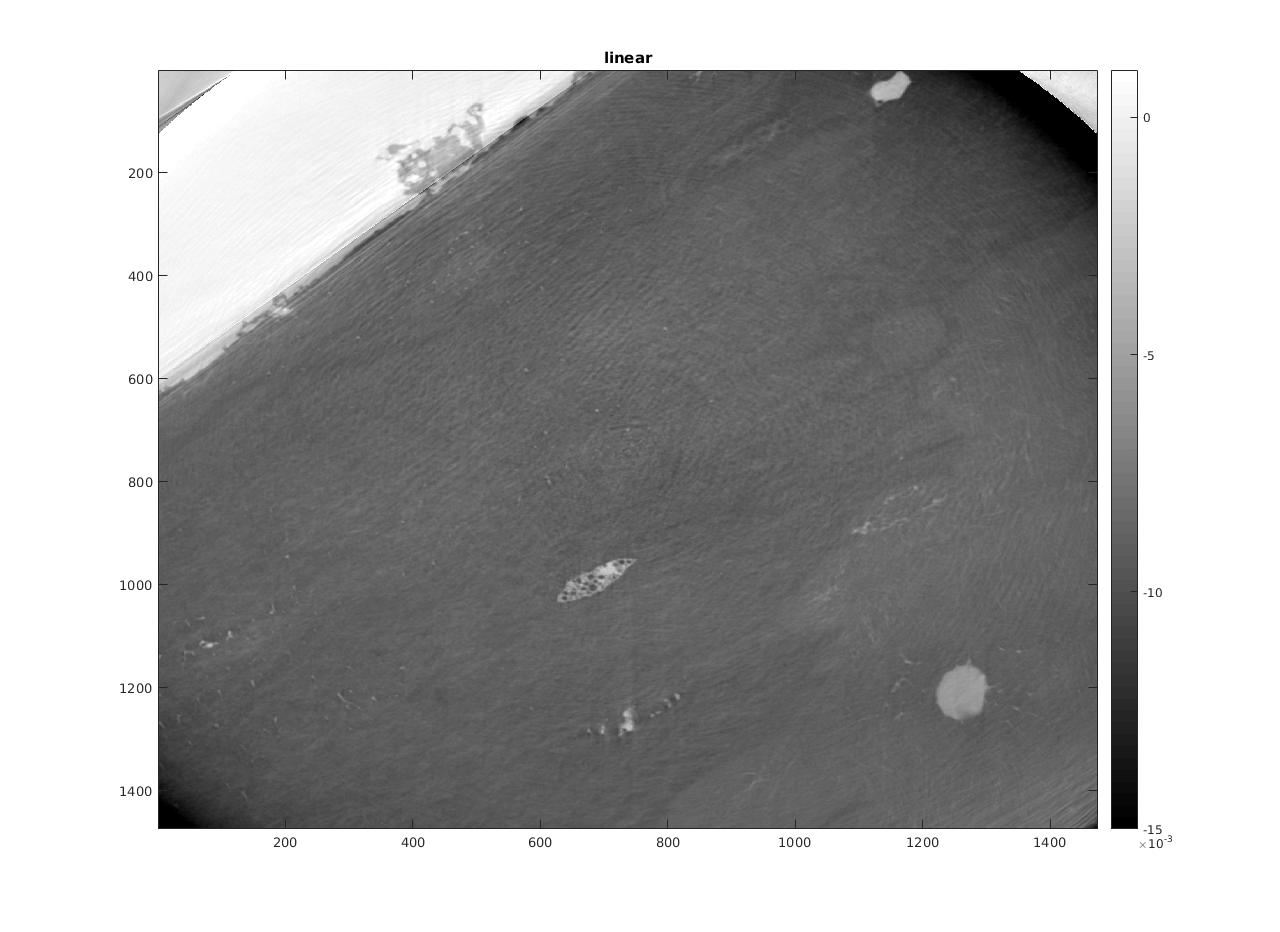
\includegraphics[width=\textwidth]{interp/linear.png}   
            \caption{Linear interpolation}
            \label{linear}
        \end{subfigure}
        \vskip\baselineskip
        \begin{subfigure}[b]{0.475\textwidth}   
            \centering 
            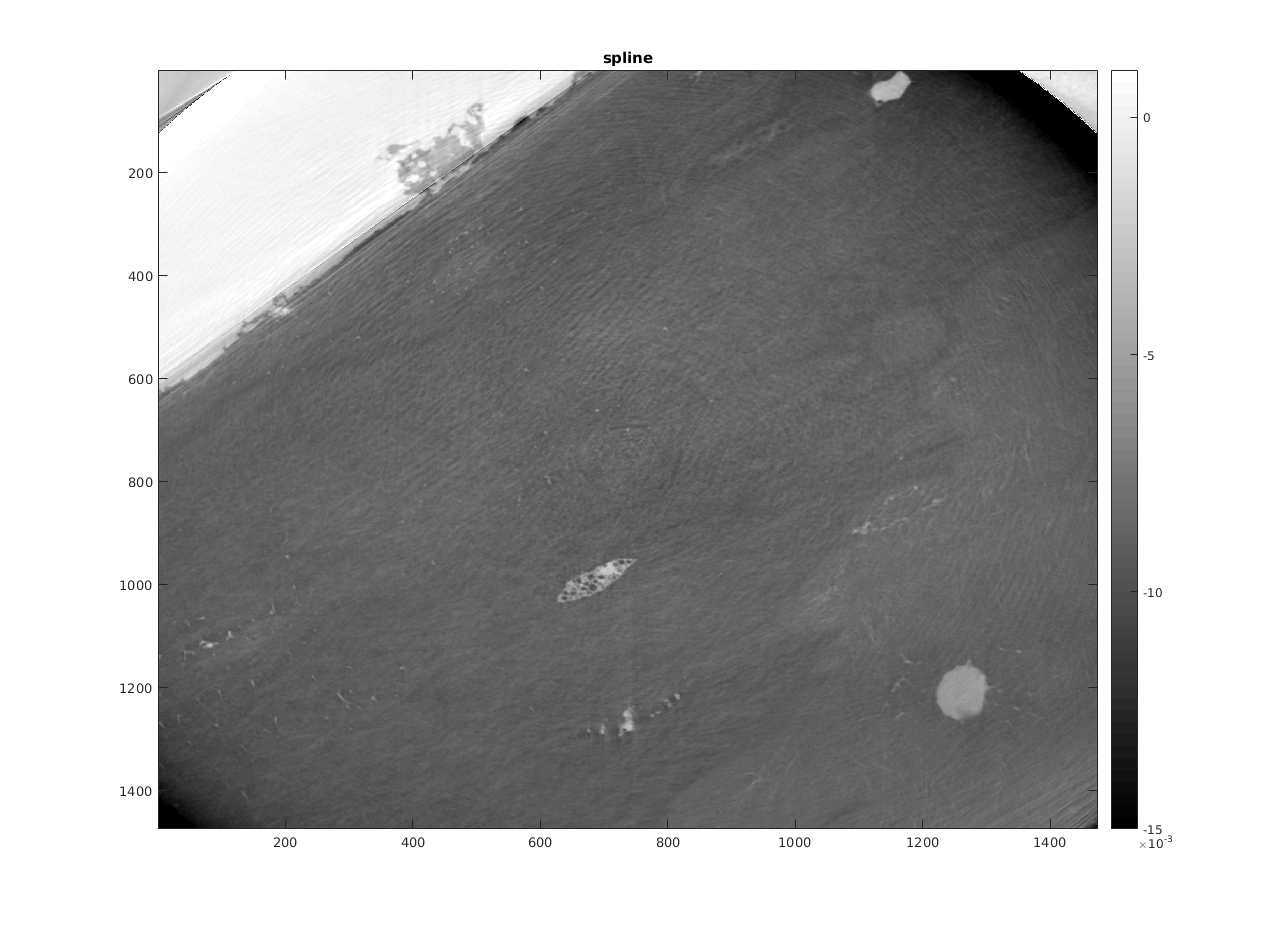
\includegraphics[width=\textwidth]{interp/spline.png}  
            \caption{Spline interpolation}
            \label{spline}
        \end{subfigure}
        \quad
        \begin{subfigure}[b]{0.475\textwidth}   
            \centering 
            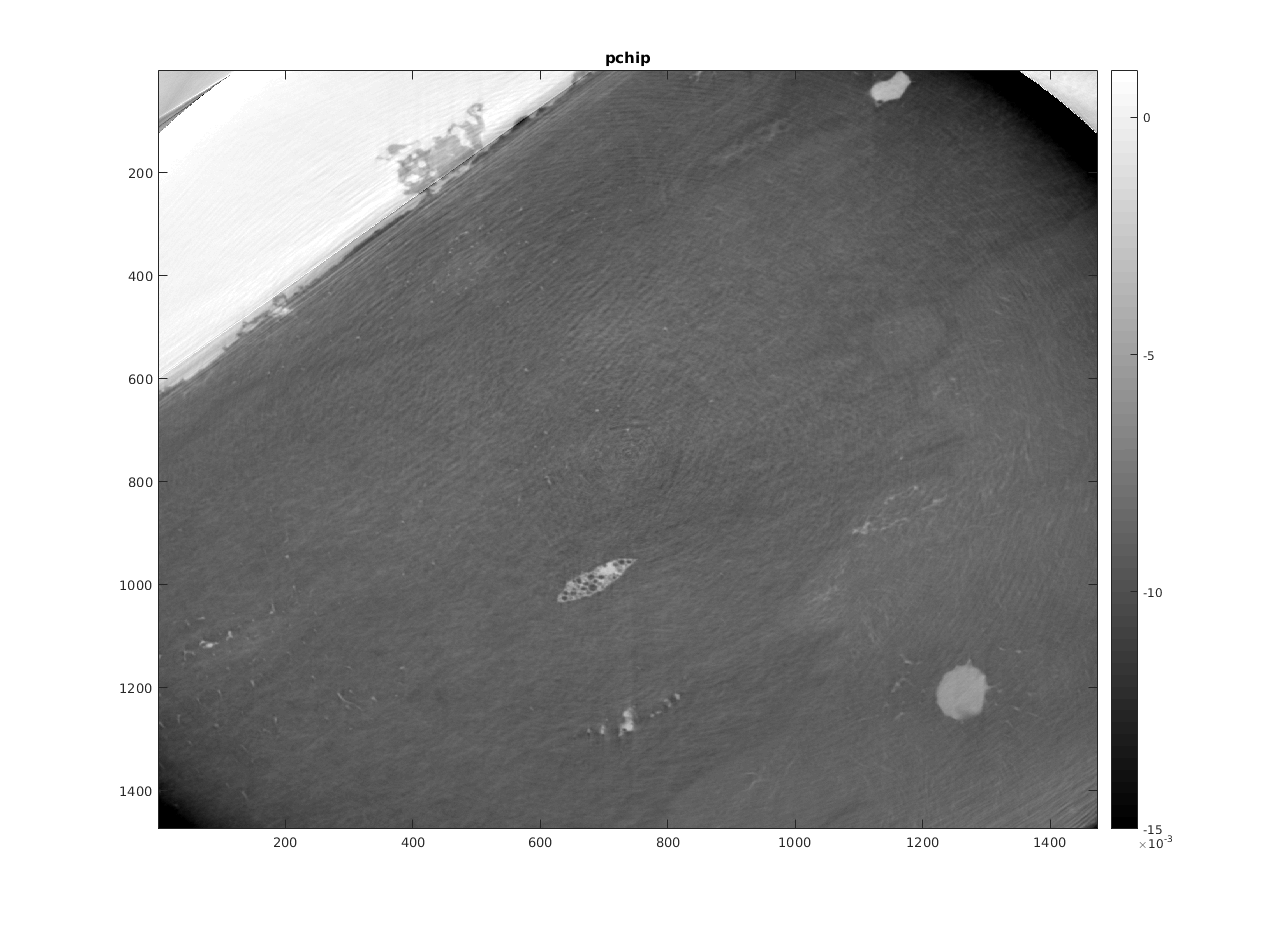
\includegraphics[width=\textwidth]{interp/pchip.png}   
            \caption{Shape-preserving piecewise cubic interpolation}
            \label{pchip}
        \end{subfigure}
        
         \vskip\baselineskip
        \begin{subfigure}[b]{0.475\textwidth}   
            \centering 
            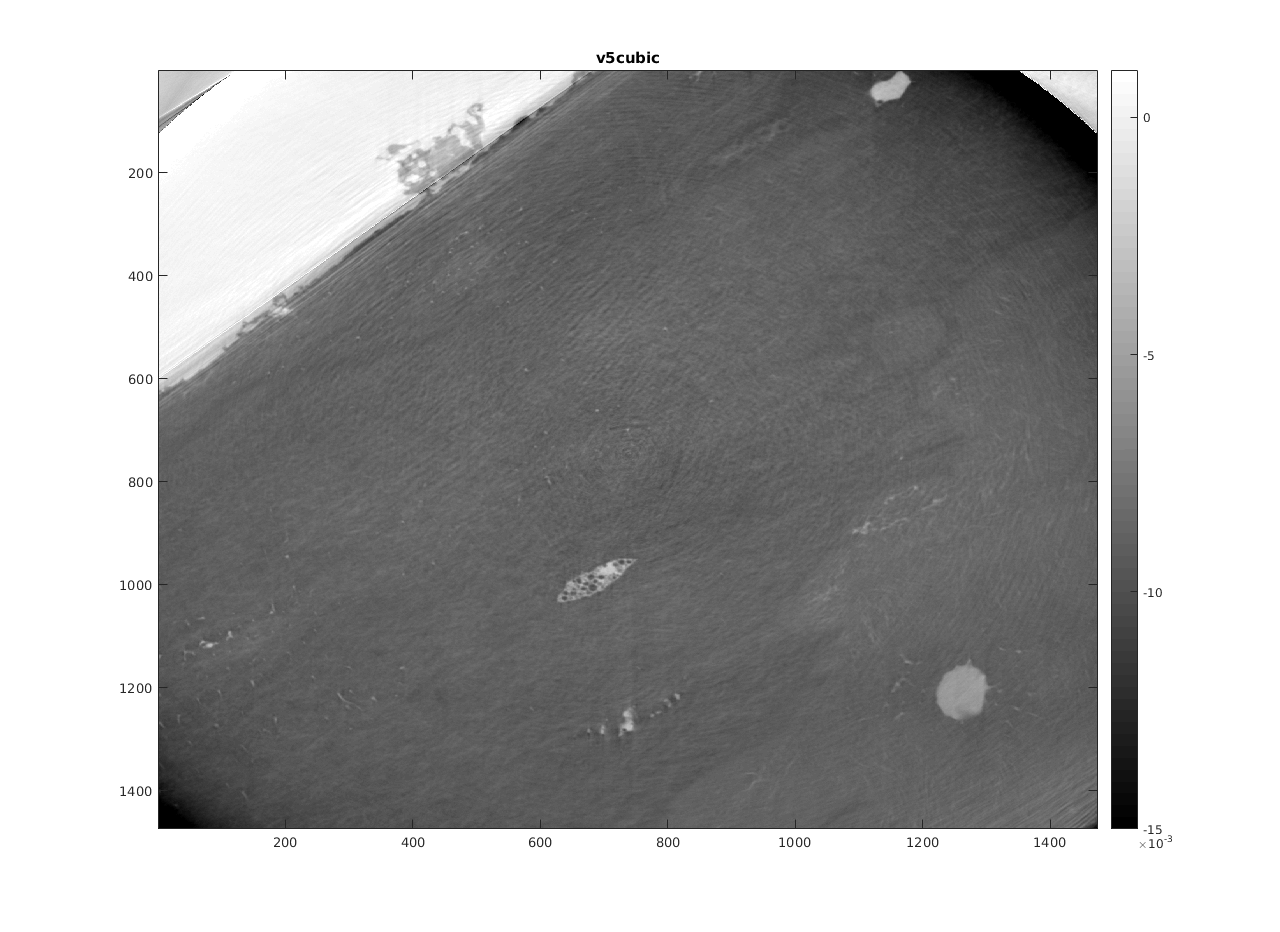
\includegraphics[width=\textwidth]{interp/v5cubic.png}   
            \caption{Cubic interpolation from MATLAB 5.}
            \label{v5cubic}
        \end{subfigure}
        
        \caption{Multiple interpolation methods for FBP with 2000 projections Slice 1001}
        \label{fig:filters}
    \end{figure}
			
	\clearpage


		\subsection{Reduced number of projections}
		A decreasing number of projections were used to perform FBP. Results were displayed in Figure \ref{fig:proj} and zoomed in Figure \ref{fig:proj}. From this figure we can notice the increase of artifact and loss of details with lower number of projections. This motivates the study of iterative reconstruction.
		
		
		\begin{figure}[h!]
        \centering	
			\begin{subfigure}[b]{0.475\textwidth}
            \centering
            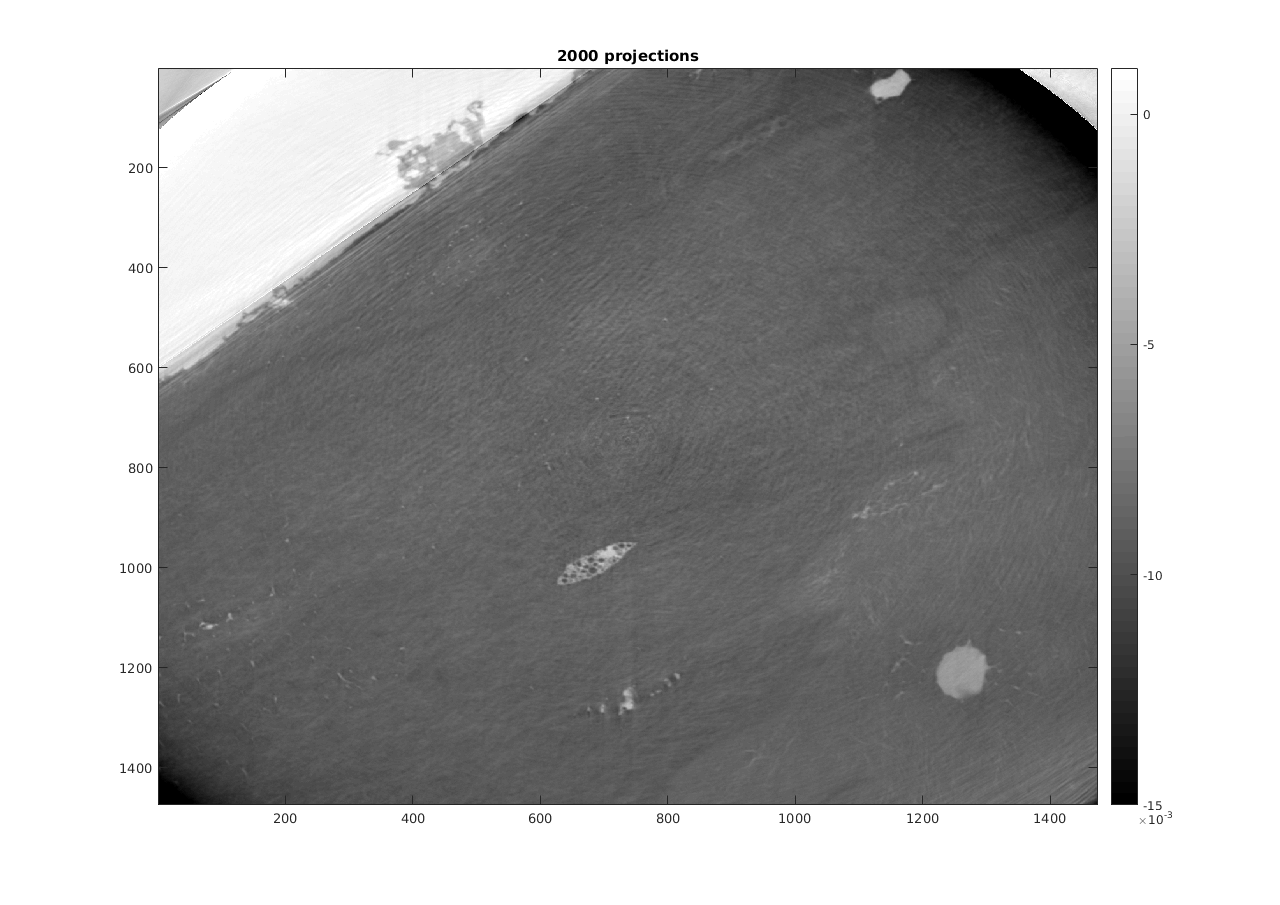
\includegraphics[width=\textwidth]{proj/2000.png}  
            \caption{Reference image 2000 projections} 
            \label{2000}
        \end{subfigure}
        \hfill
        \begin{subfigure}[b]{0.475\textwidth}  
            \centering 
            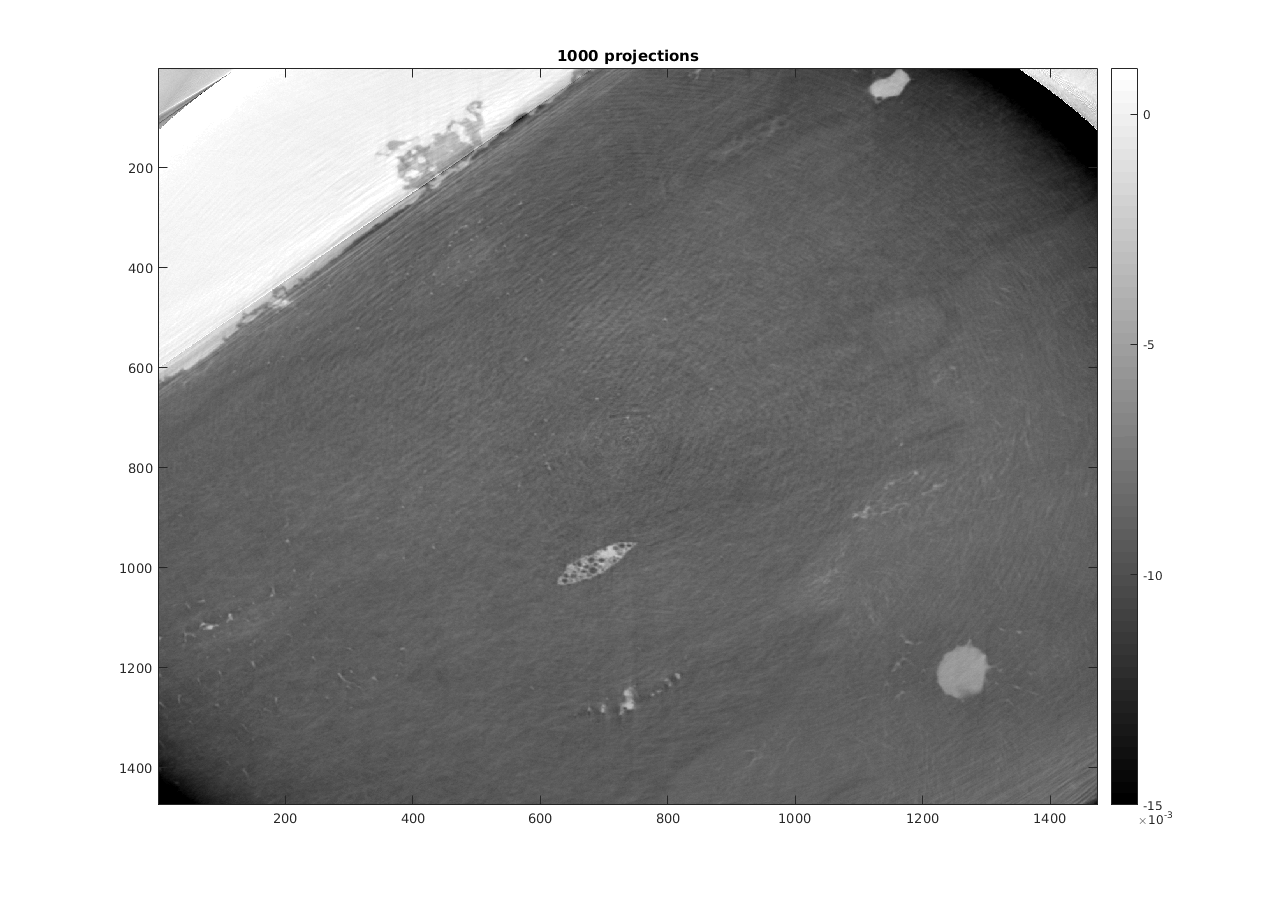
\includegraphics[width=\textwidth]{proj/1000.png}   
            \caption{1000 projections}
            \label{1000}
        \end{subfigure}
        \vskip\baselineskip
        \begin{subfigure}[b]{0.475\textwidth}   
            \centering 
            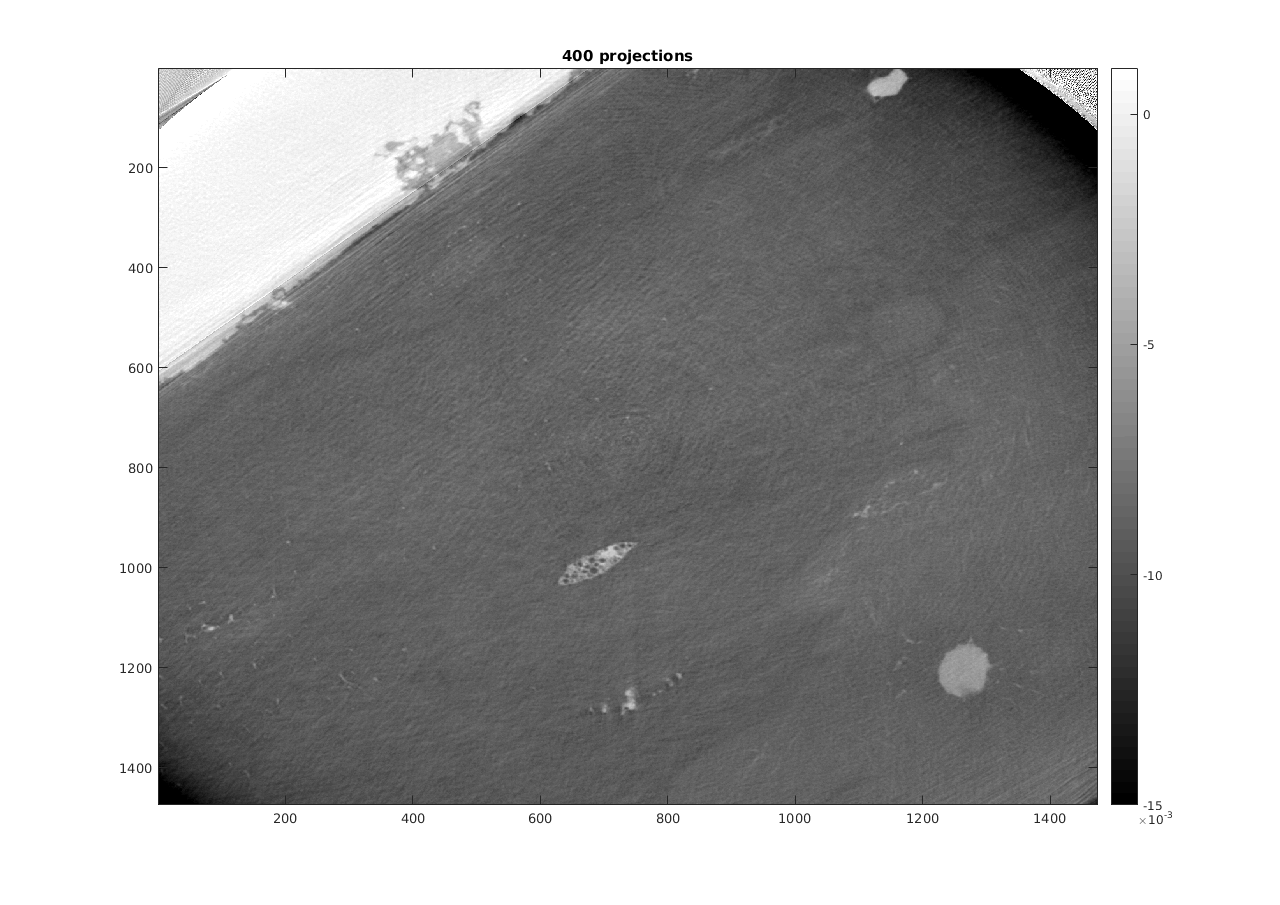
\includegraphics[width=\textwidth]{proj/400.png}  
            \caption{400 projections}
            \label{400}
        \end{subfigure}
        \quad
        \begin{subfigure}[b]{0.475\textwidth}   
            \centering 
            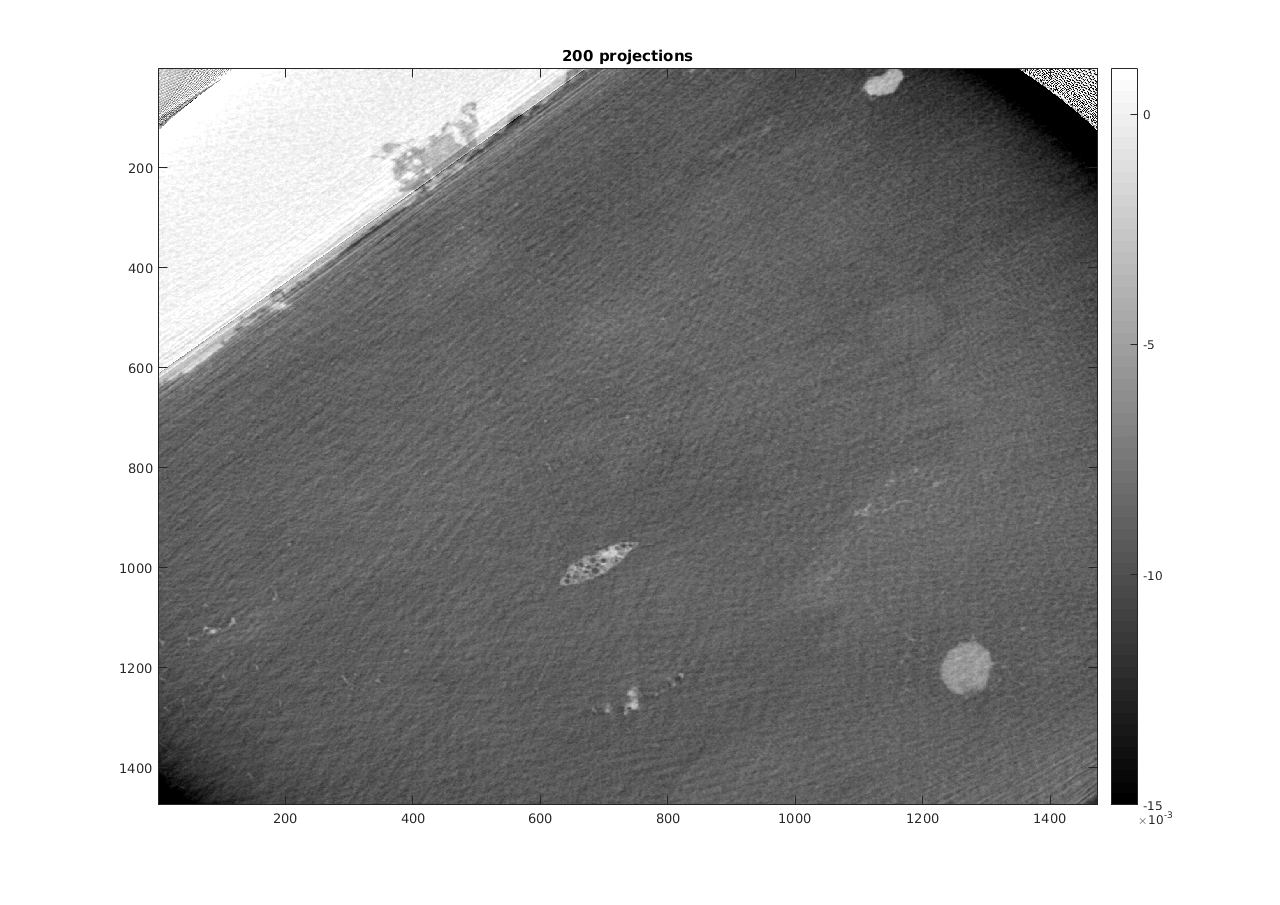
\includegraphics[width=\textwidth]{proj/200.png}   
            \caption{200 projections}
            \label{200}
        \end{subfigure}
        
         \vskip\baselineskip
        \begin{subfigure}[b]{0.475\textwidth}   
            \centering 
            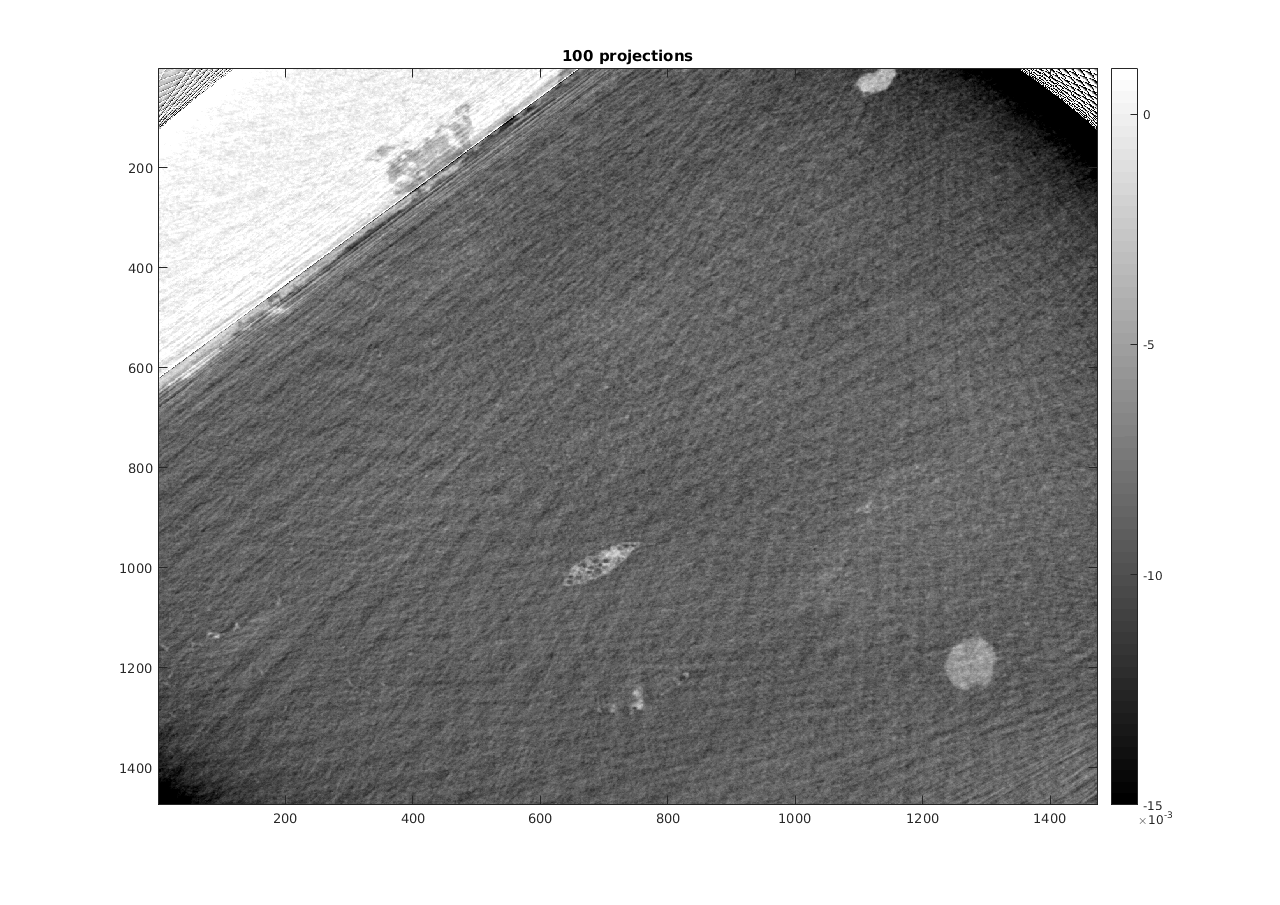
\includegraphics[width=\textwidth]{proj/100.png}   
            \caption{100 projections}
            \label{100}
        \end{subfigure}
        
        \caption{Multiple number of projection for FBP on Slice 1001}
        \label{fig:proj}
    \end{figure}
    
    \begin{figure}[h!]
        \centering	
			\begin{subfigure}[b]{0.475\textwidth}
            \centering
            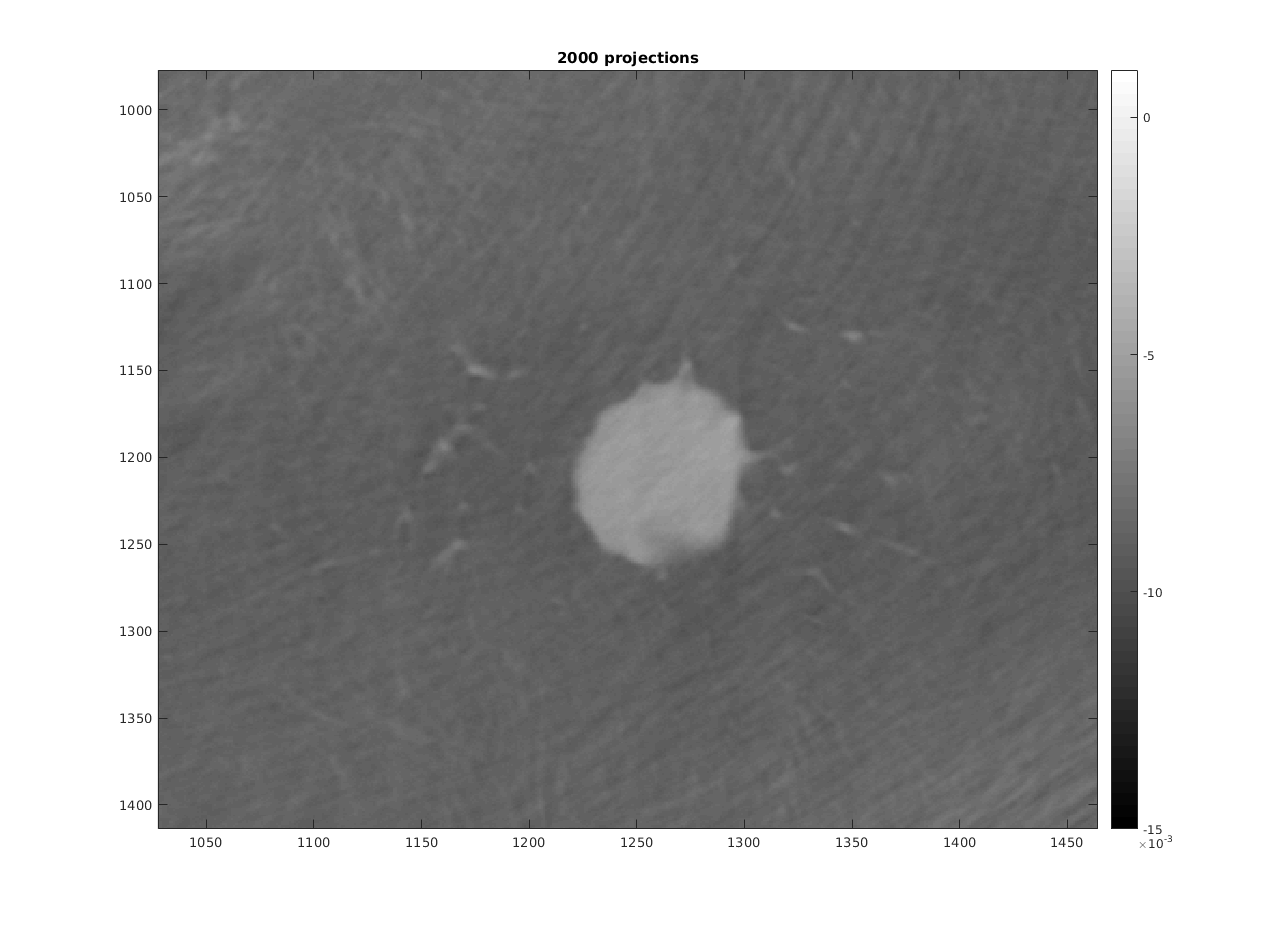
\includegraphics[width=\textwidth]{proj/ZOOMED/2000.png}  
            \caption{Reference image 2000 projections} 
            \label{2000Z}
        \end{subfigure}
        \hfill
        \begin{subfigure}[b]{0.475\textwidth}  
            \centering 
            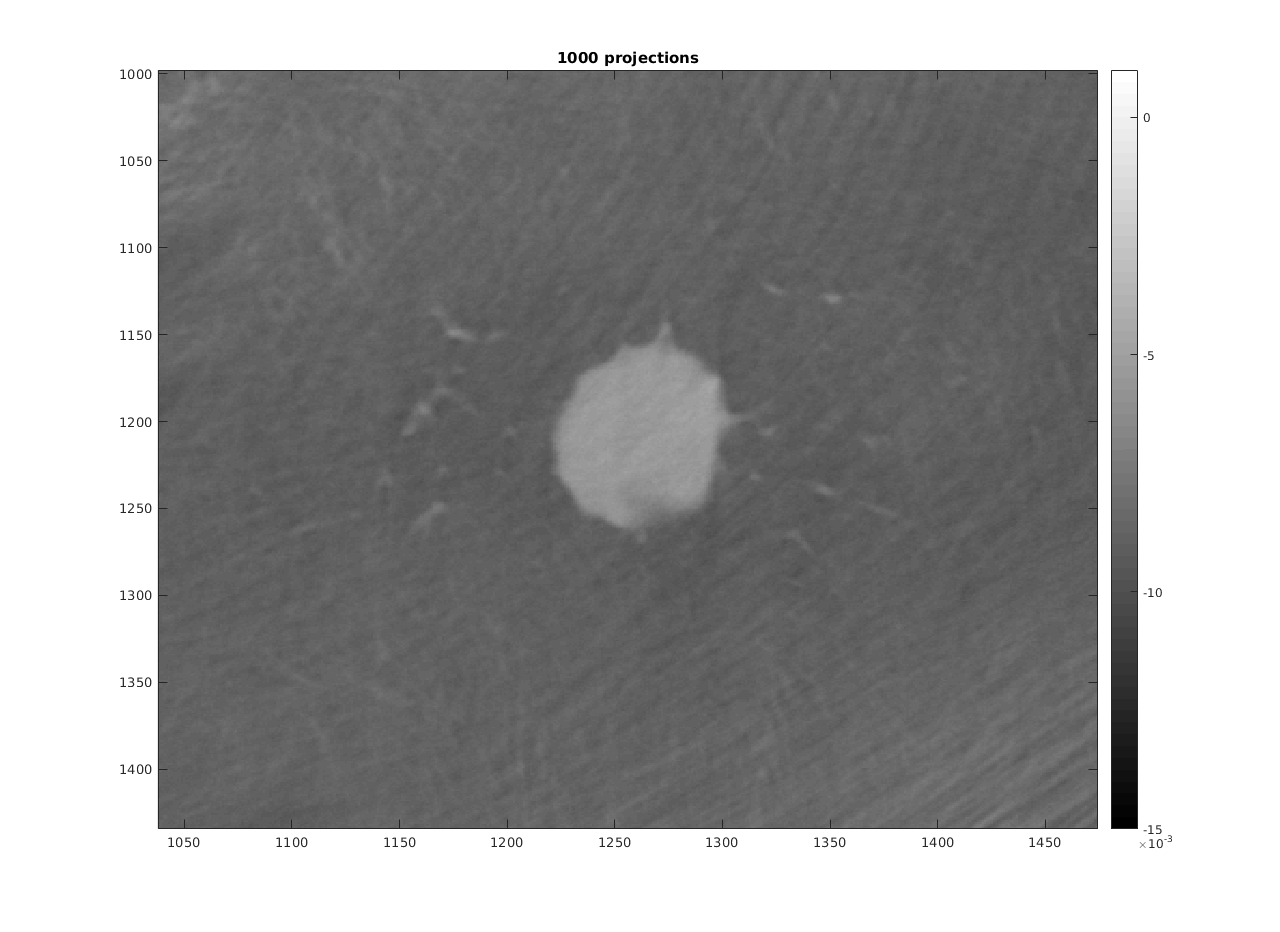
\includegraphics[width=\textwidth]{proj/ZOOMED/1000.png}   
            \caption{1000 projections}
            \label{1000Z}
        \end{subfigure}
        \vskip\baselineskip
        \begin{subfigure}[b]{0.475\textwidth}   
            \centering 
            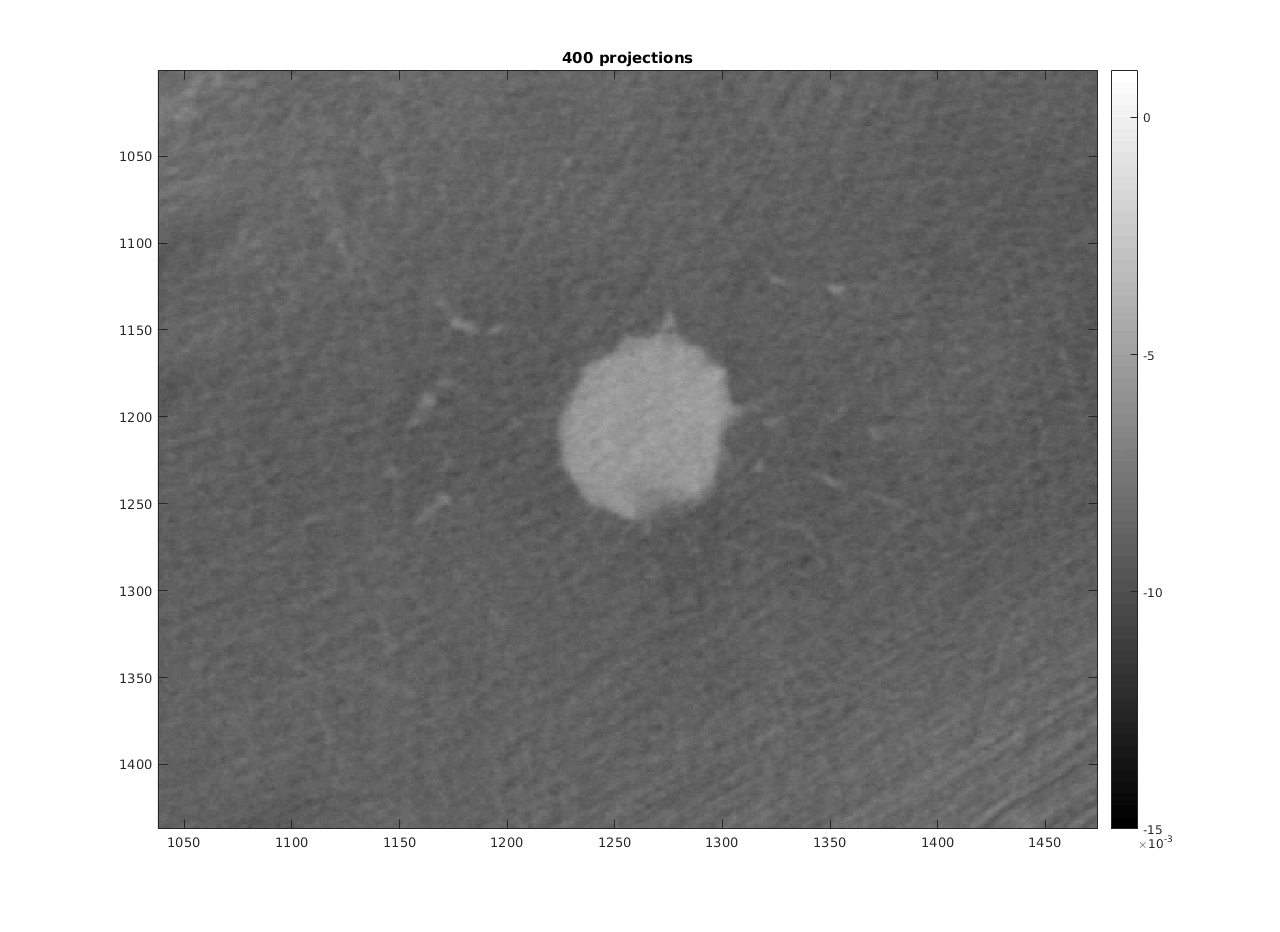
\includegraphics[width=\textwidth]{proj/ZOOMED/400.png}  
            \caption{400 projections}
            \label{400Z}
        \end{subfigure}
        \quad
        \begin{subfigure}[b]{0.475\textwidth}   
            \centering 
            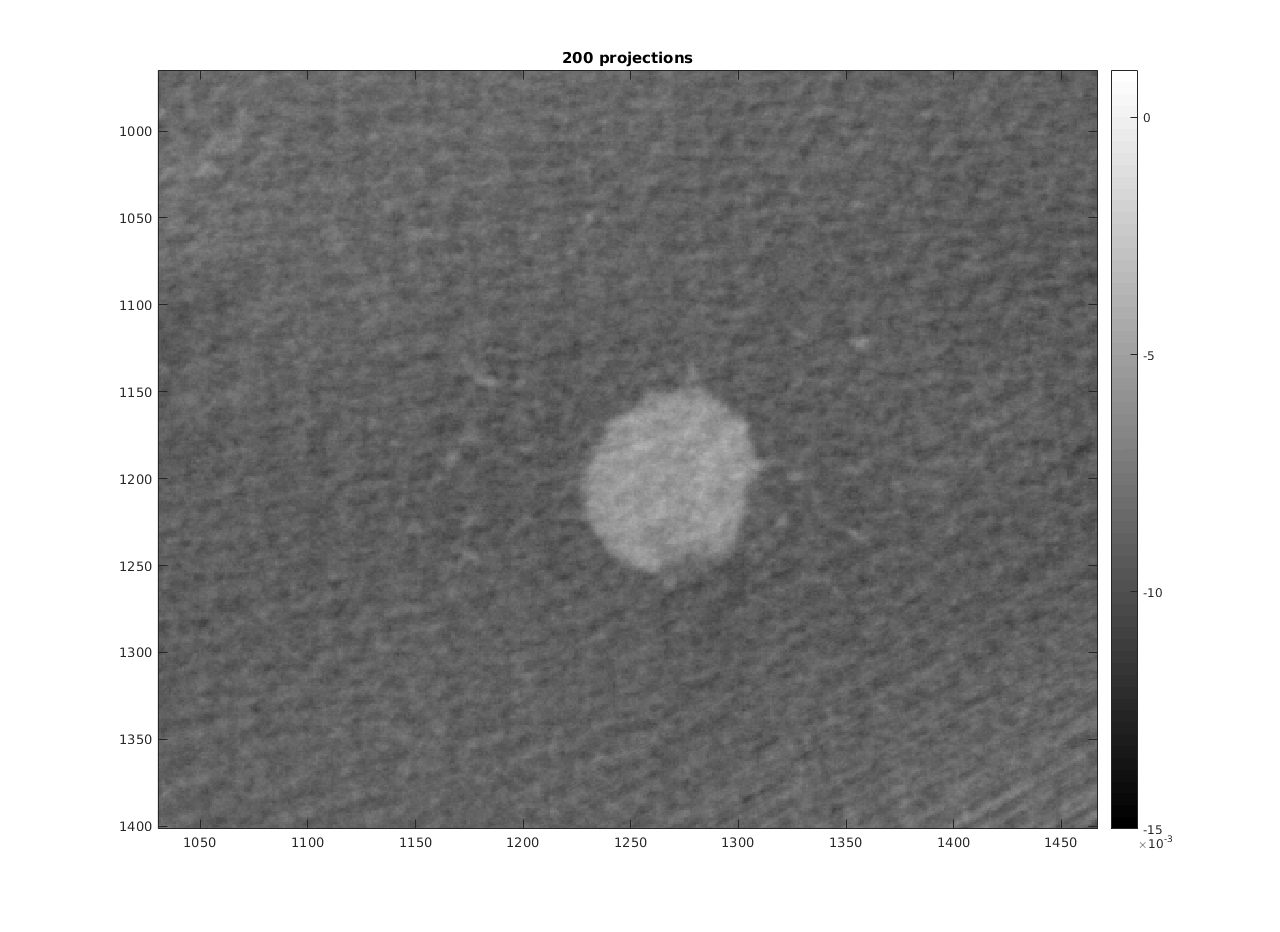
\includegraphics[width=\textwidth]{proj/ZOOMED/200.png}   
            \caption{200 projections}
            \label{200Z}
        \end{subfigure}
        
         \vskip\baselineskip
        \begin{subfigure}[b]{0.475\textwidth}   
            \centering 
            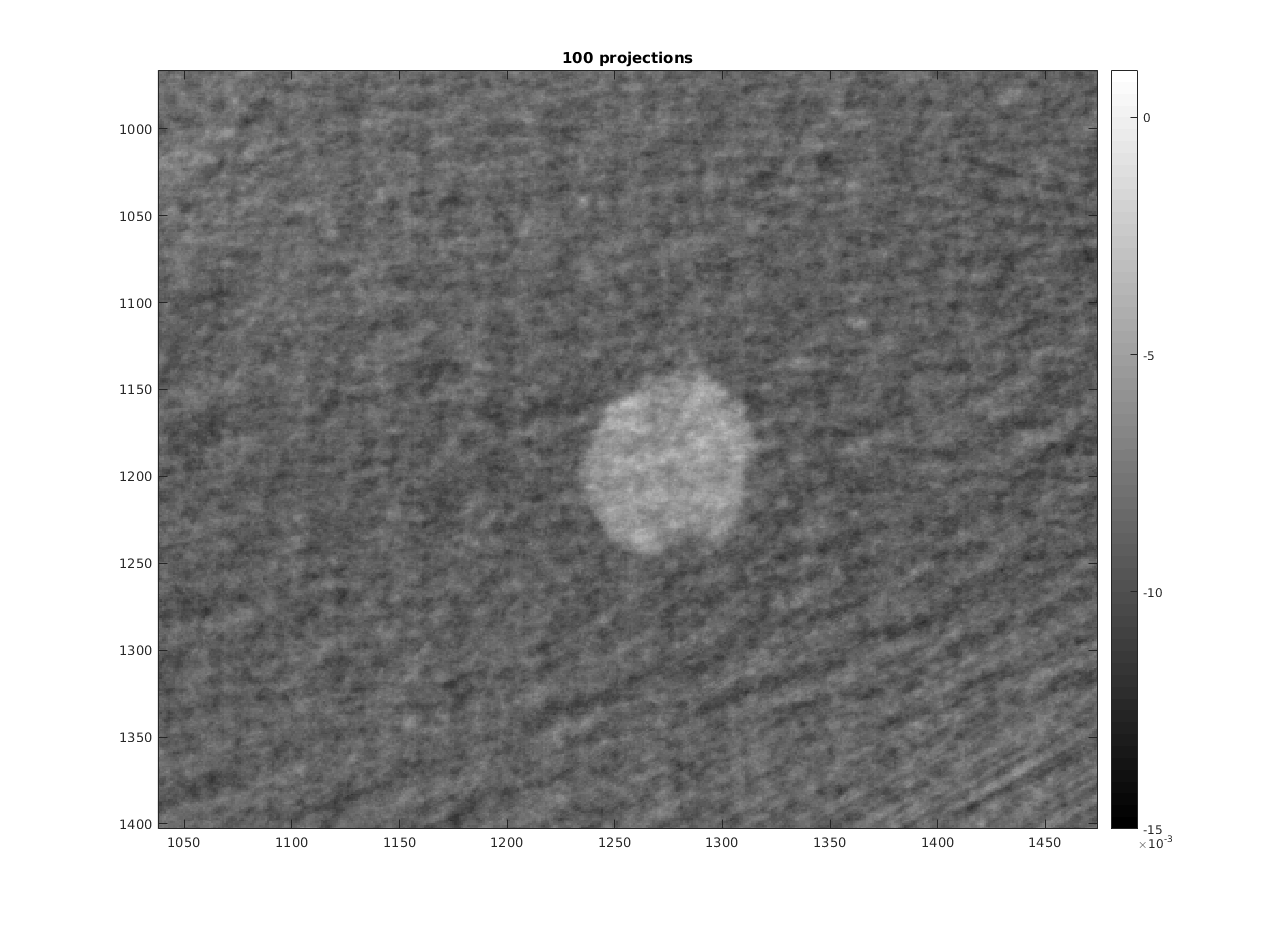
\includegraphics[width=\textwidth]{proj/ZOOMED/100.png}   
            \caption{100 projections}
            \label{100Z}
        \end{subfigure}
        
        \caption{Multiple number of projection for FBP on Slice 1001 zoomed}
        \label{fig:projZ}
    \end{figure}
    
	\clearpage
\section{iterative reconstruction}	
currently working on Split-Bregman method.
\section{Index}
	\subsection{Sinogram}
		\label{SinoImg}
		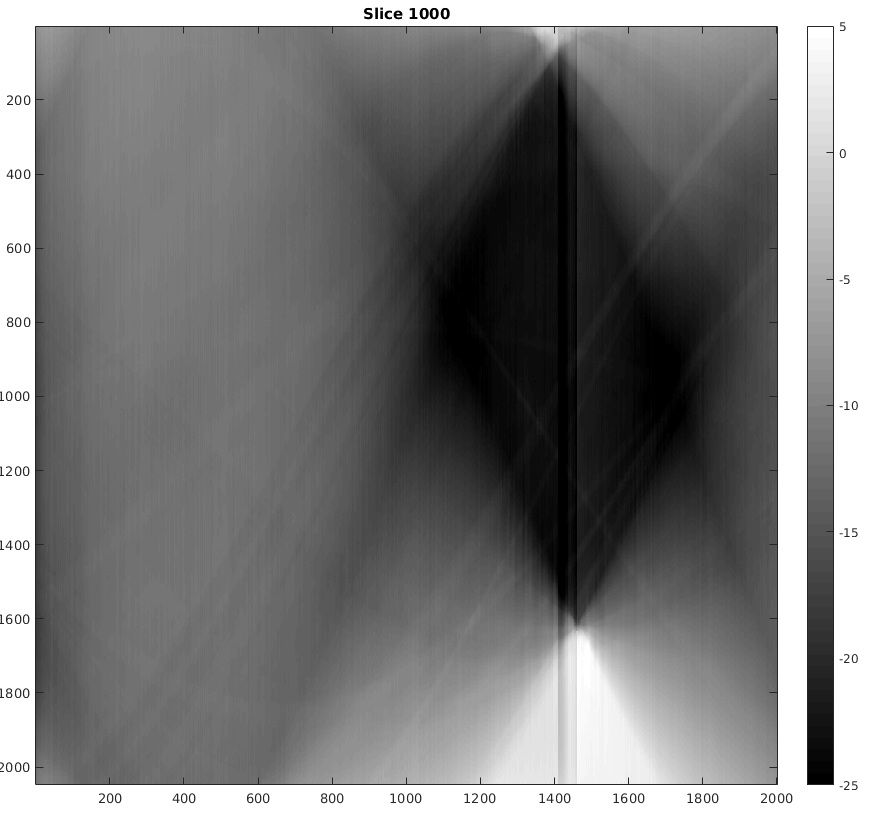
\includegraphics[width=\textwidth]{sinograms/Slice1000.png}
		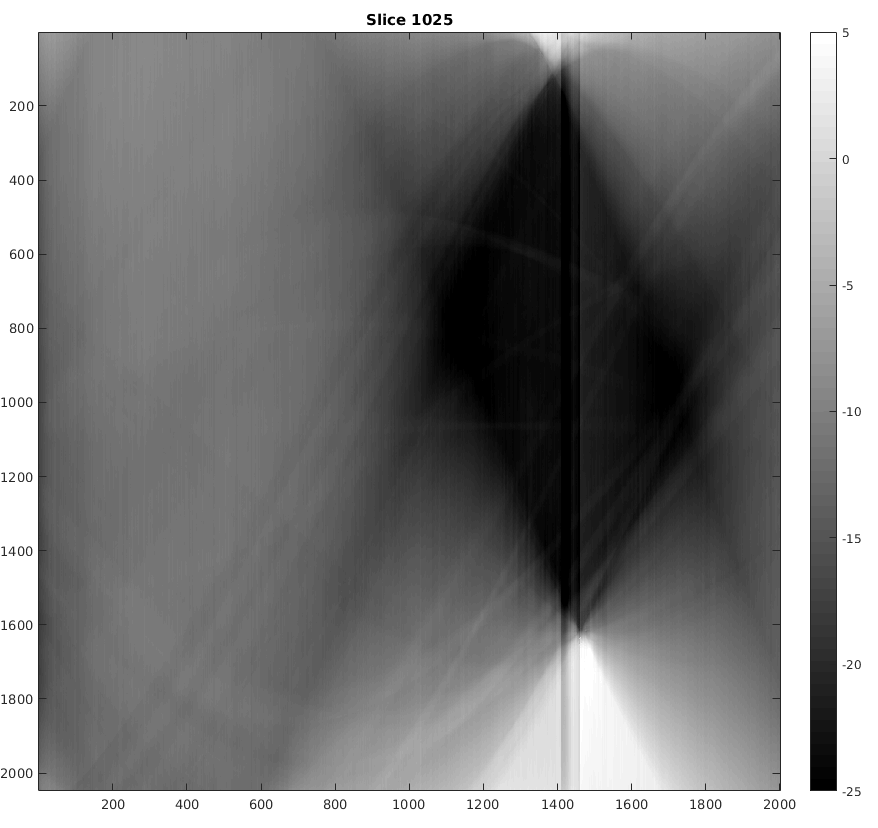
\includegraphics[width=\textwidth]{sinograms/Slice1025.png}
		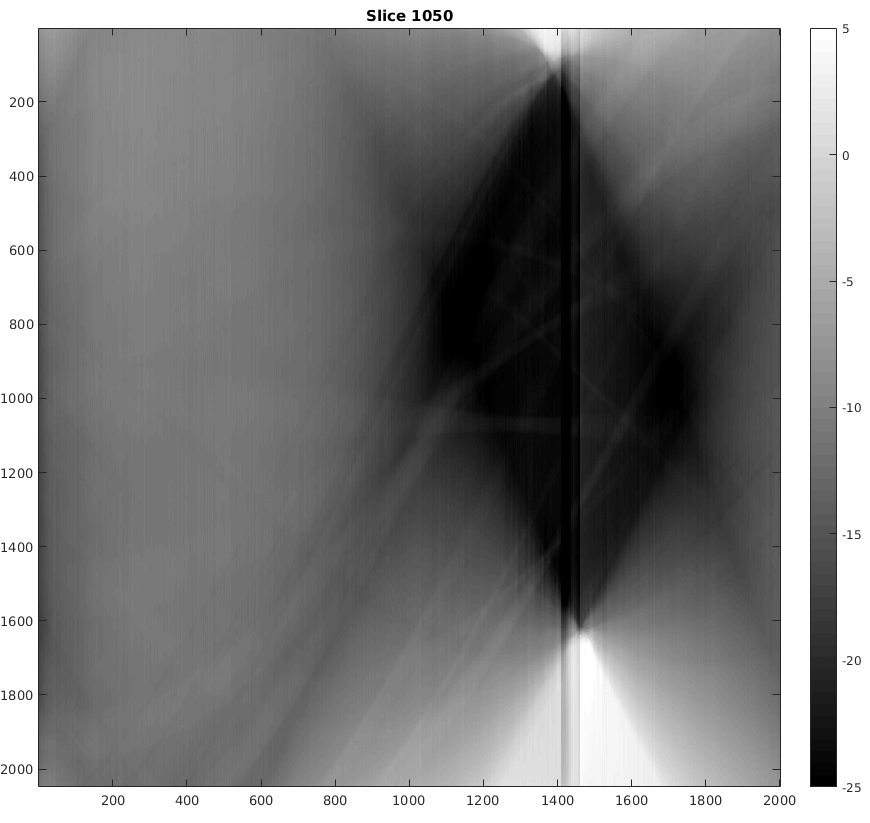
\includegraphics[width=\textwidth]{sinograms/Slice1050.png}
		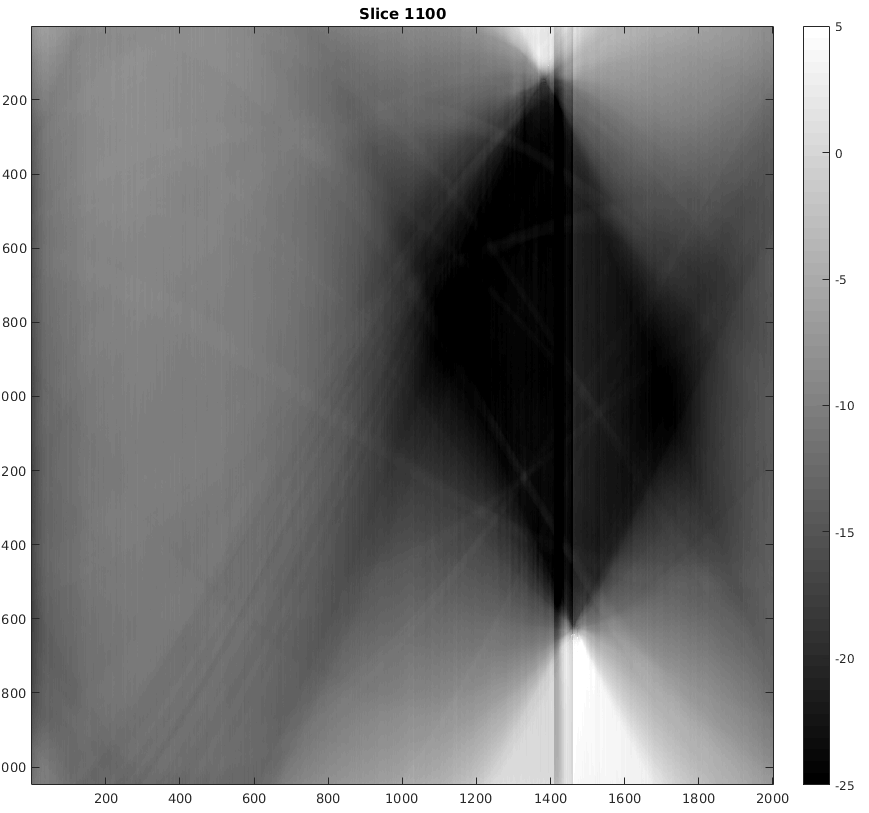
\includegraphics[width=\textwidth]{sinograms/Slice1100.png}
    \subsection{Without zero padding}
        \label{wtout0pad}
        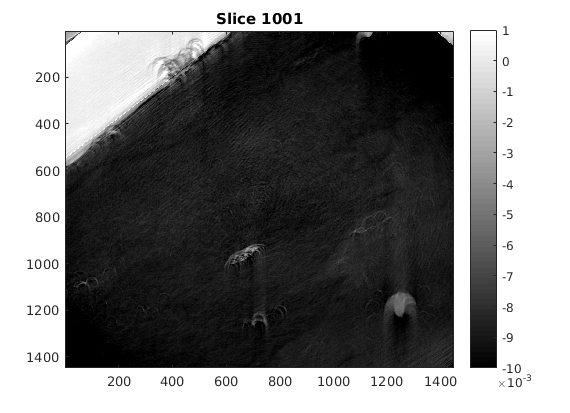
\includegraphics[width=\textwidth]{no0pad/slice1001.png}
        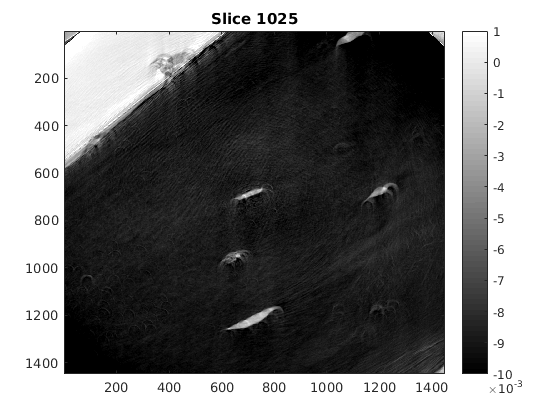
\includegraphics[width=\textwidth]{no0pad/slice1025.png}
        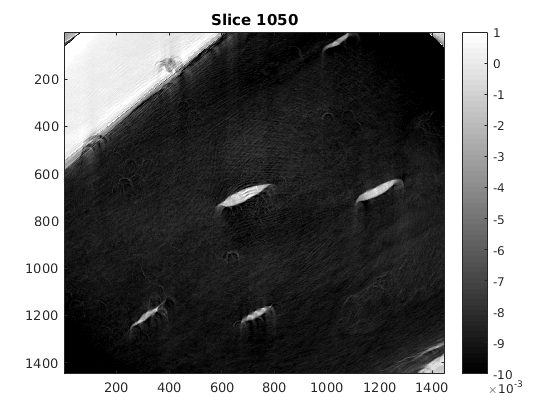
\includegraphics[width=\textwidth]{no0pad/slice1050.png}
        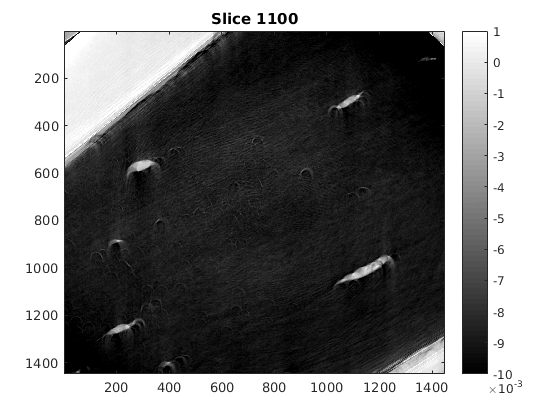
\includegraphics[width=\textwidth]{no0pad/slice1100.png}
\end{document}